\documentclass{lib/styles/default-style}

\begin{document}
\pagestyle{default-numbered}
\startPageCountFrom{5}

\tableofcontents

\newpage

\unnumberedSection{ПЕРЕЛІК УМОВНИХ СКОРОЧЕНЬ}

    PoW --- Proof of Work

    PoS --- Proof of Stake

    DPoS --- Delegated Proof of Stake

    BFT --- Byzantine Fault Tolerance
    
    PBFT --- Practical Byzantine Fault Tolerance
    
    HBBFT --- Honey Badger Byzantine Fault Tolerance
    
    PEG --- Parsing expression grammar
    
    CFG --- Context free grammar
    
    VM --- Virtual Machine
    
    PVM --- Program virtual machine
    
    MRE --- Managed runtime environment
    
    ISA --- Instruction set architecture

    EVM --- Ethereum Virtual Machine

    RPC --- Remote Procedure Call

    REST --- Representational State TransferI/O

    I/O --- Input/Output operations

\newpage

\unnumberedSection{ВСТУП}

    З кожним роком кількість інформації непреривно збільшується, а кількість цифрової інформації і поготів,
    та, судячи з усього, ця тенденція не планує припинятися. Із ростом кількості цифрової інформації, зростає і
    кількість ресурсів, необхідних для обробки цієї інформації. Хоча вартість цих ресурсів непреривно зменшується,
    проте великі системи потребують чимало коштів. Системи стають складнішими, необхідно ще більше потужностей для обробки інформації.

    Такі системи складно підтримувати, саме тому і почався пошук альтернативних рішень. В останній час все більше людей дивиться у бік
    децентралізованих рішень. Проте, у існуючих рішень є проблеми із масштабованість та швидкістю транзакцій в тому, чи іншому вигляді.

    Вирішення даних проблем може кардинально змінити укореніле уявлення про системи обробки інформації, та дати поштовх до створення
    більш оптимальних систем.

    Результати можуть бути використані у всіх галузях виробництва, де тим чи іншим чином оброблюється інформація.
    Саме тому обрана проблематика дослідження є вельми актуальною на даний момент.

    Метою даної магістерської дисертації є дослідження концепцій для створення гнучкої платформи для розробки швидких децентралізованих додатків
    та реалізація прототипу платформи. Проаналізувати існуючі платформи, запропонувати алгоритм консенсусу  даних  в  розподілених  системах,
    алгоритм сереалізації даних, механізми для оптимізації використання ресурсів в децентралізованих системах,
    спроектувати  систему  котра  підтримує запропоновані концепції.

    Відповідно до мети роботи необхідно вирішити такі завдання:
    \listDefault{
        \item розглянути поняття про платформи для створення децентралізованих додатків;
        \item описати устрій спроектованої системи для розробки блокчейн додатків;
        \item описати реалізацію запропонованих концепцій;
        \item навести результати випробовування розробленого рішення;
        \item розробити стартап-проект.
    }

    Об'єкт дослідження – платформи для створення децентралізованих додатків.

    Предметом дослідження є концепції побудови децентралізованих додатків, які дозволяють створювати ефективні рішеня.

    Основним здобутком дисертації є методологія проектування алгоритму консесусу, для
    швидкого та надійного обміну даними у децентралізованих мережах,
    проектування алгоритму пошуку вузлів, для стабілізації децентралізованої системи та
    проектування механізмів використання ресурсів для підтримки децентралізованих додатків, зокрема
    проектування та оптимізація програмних віртуальних машин для виконання криптографічних операцій
    та оптимізація механізма виконання I/O операцій. 

    Отримана в результаті виконаної дослідницької роботи методологія
    оптимізації були опубліковані у статті «ЗАХИЩЕНА P2P КОМУНІКАЦІЯ НА ОСНОВІ ТЕХНОЛОГІЇ BLOCKCHAIN» в
    сучасному науковому журналі «Інформаційне суспільство: технологічні,
    економічні та технічні аспекти становлення» в 2019 році.

\startSection{АНАЛІЗ ІСНУЮЧИХ ПЛАТФОРМ ДЛЯ СТВОРЕННЯ ДЕЦЕНТРАЛІЗОВАНИХ ДОДАТКІВ}

\subsection{Платформа для створення додатків Ethereum}

    Платформа для створення практично будь-яких децентралізованих
    онлайн-сервісів на базі блокчейна (Đapps), що працюють на базі розумнихĐapps), що працюють на базі розумних), що працюють на базі розумних
    контрактів. Реалізована як єдина децентралізована віртуальна машина. Ідея була
    втілена 30 липня 2015 року. Оскільки Ethereum сильно спрощує і здешевлює
    впровадження блокчейна, його впроваджують як великі гравці, такі як Microsoft, IBM, Acronis,
    Сбербанк, банківський консорціум R3, так і нові стартапи.

    У кінці 2013 року Ethereum запропонував дослідник
    і програміст криптовалют Віталік Бутерін. Розвиток фінансувався через інтернет-краудфандінг, який проходив
    у липні-серпні 2014 року. Потім система вийшла у світ 30 липня 2015 року, при цьому 72 мільйони монет були
    створені "попередньо". Це становить близько 68 відсотків загального обсягу постачання у 2019 році [1]. 

    У 2016 році,
    внаслідок експлуатації вразливості в програмному забезпеченні проекту, та подальшого розкрадання ефіру на суму 
    50 мільйонів доларів, Ethereum було розділено на дві окремі блокчейн --- нова окрема версія стала Ethereum (ETH), а оригінал продовжувався 
    як Ethereum Classic (ETC).

    Ethereum є дуже потужною платформою розробки через технологію розумних контрактів

    Розумний контракт --- це код, який працює на EVM.
    Смарт-контракти можуть приймати та зберігати ефір, дані або комбінацію обох.
    Потім, використовуючи логіку, запрограмовану в договорі, він може поширювати
    цей ефір на інші рахунки або навіть інші смарт-контракти.

    Як приклад, приведемо відомий контракт з Бобом та Алісою (рисунок \ref{img:alice-bob-contract-example}). Аліса хоче найняти Боба, щоб побудувати їй внутрішній дворик,
    і вони використовують контракт для депонування (місце для зберігання грошей, доки умова не буде виконана),
    щоб зберігати свій ефір до остаточної транзакції.

    \printImage[1][0.3]{alice-bob-contract-example}{Приклад виконання розумного контракта Боба та Аліси}

    Розумні контракти пишуться мовою, що називається "Solidity". Solidity має статичний тип і підтримує механізм успадкування,
    бібліотеки та складні,визначені користувачем типи. Синтаксис Solidity схожий на JavaScript [2].

    Програми, що використовують смарт-контракти для їх обробки, називаються "децентралізованими програмами"\enspace або "dapps".
    Користувацькі інтерфейси для цих daaps складаються з відомих мов, таких як HTML, CSS та JavaScript.
    Саму програму можна розмістити на традиційному веб-сервері або на децентралізованій файловій службі, наприклад, Swarm або IPFS.

    Враховуючи переваги блокчейна Ethereum, dapp може бути рішенням для багатьох галузей, включаючи, але не обмежуючись ними:

    \listDefault{
        \item бухгалтерський облік;
        \item фінанси;
        \item логістика;
        \item нерухомість;
        \item електронні магазиги (маркетплейси).
    }

\subsection{Платформа для створення додатків Hyperledger}

    Комплексний проект розробки блокчейну з відкритим вихідним кодом та пов'язаних з цим інструментів,
    який було розпочато Linux Foundation у грудні 2015 року. Основною метою проекту є підтримка спільної
    розробки мереж з розподіленим реєстром, заснованих на технології блокчейн.
    
    У грудні 2015 року Linux Foundation анонсувала створення проекту Hyperledger.
    Імена компаній-засновників були оголошені у лютому 2016, до яких 29 березня того ж року приєдналися ще
    десять учасників і було затверджено склад ради правління. 29 травня виконавчим директором проекту призначили Брайана Белендорфа [3].
    
    Метою проекту є посилення міжгалузевої співпраці за допомогою технології блокчейну та мереж з розподіленим реєстром.
    Особлива увага приділяється підвищенню продуктивності та надійності цих систем (у порівнянні з аналогічними криптовалютними розробками),
    аби вони могли використовуватися технологічними, фінансовими та компаніями-постачальниками в масштабах глобальних комерційних оборудок. 
    
    Проект поєднуватиме незалежні відкриті стандарти та протоколи за допомогою фреймворків для створення специфічних модулей, включно з 
    блокчейнами з власними механізмами досягнення консенсусу та порядком збереження даних, а також ідентифікаційними сервісами, контролем
    доступу та смарт-контрактами. 	Попри чутки, згідно з заявою Брайана Белендорфа, введення та використання власної криптовалюти у проекті
    ніколи не відбудеться.
    
    На початку 2016 проект розпочав розглядати пропозиції щодо створення вихідного коду
    та інших ключових технологічних елементів. Однією з перших пропозицій було поєднати попередні розробки Digital Asset,
    механізм досягнення консенсусу від Blockstream та OpenBlockchain від IBM. Пізніше ця технологія отримала назву Fabric (рисунок \ref{img:hyperledger-struct}).
    
    \printImage[1][0.7]{hyperledger-struct}{Структурна схема платформи Hyperledger Fabric}

    У травні розпочалася розробка мережі з розподіленим реєстром Sawtooth від Intel. 

    12 червня 2017 року проект анонсував готову до промислового використання версію Hyperledger Fabric 1.0 який одразу 
    почав набирати популярність на ринку ICO. Того ж місяця London Stock Exchange Group, спільно з IBM, заявила про початок
    розробки блокчейн-платформи на базі Hyperledger Fabric для випуску цифрових акцій італійських компаній. 
    
    У серпні 2017, компанія Oracle приєдналася до консорціуму Hyperledger і  оголосила про початок розробки власного хмарного блокчейн-сервісу. 
    
    У вересні 2017 Королівський банк Канади почав використовувати Hyperledger для міжбанківських розрахунків з США. 
   
    Hyperledger забезпечує такі функціональні можливості для мережі:
    
    \listDefault{
        \item управління ідентичністю --- Hyperledger Fabric надає послугу посвідчення членства,
        яка керує ідентифікаторами користувачів та аутентифікує всіх учасників мережі, 
        списки контролю доступу можуть використовуватися для надання додаткових рівнів дозволу через авторизацію конкретних
        мережевих операцій;
        \item приватність та конфідейційність --- Hyperledger дозволяє конкуруючим інтересам бізнесу
        та будь-яким групам, які потребують приватних, конфіденційних транзакцій, співіснувати в одній і тій же дозволеній мережі, через
        приватні канали, які представляють із себе обмежені шляхи обміну повідомленнями, які можна використовувати для
        забезпечення конфіденційності та конфіденційності транзакцій для конкретних підмножин членів мережі,
        усі дані, включаючи інформацію про трансакції, учасників та каналів, на каналі є невидимими та недоступними
        для будь-яких членів мережі, яким явно не надано доступ до цього каналу;
        \item ефективна обробка --- Hyperledger Fabric призначає мережеві ролі за типом вузла,
        для забезпечення одночасності та паралелізму в мережі виконання транзакцій відокремлено
        від впорядкування та зобов'язань транзакцій. Виконання транзакцій перед їх
        замовленням дозволяє кожному вузлу однорангових обробляти одночасно кілька транзакцій,
        це одночасне виконання збільшує ефективність обробки кожного партнера та прискорює доставку транзакцій до служби замовлення;
        \item chaincode --- це визначення програмного забезпечення як активів та інструкція щодо
        транзакцій для зміни активів, chaincode виконує правила читання або зміни пар ключових
        значень або іншої інформації бази даних стану, його функції виконуються в базі даних поточного стану
        і ініціюються через пропозицію транзакцій.
    }
\subsection{Платформа для створення додатків Corda}

    Платформа з відкритим вихідним кодом, яка дозволяє підприємствам здійснювати операції безпосередньо
    та у суворій конфіденційності за допомогою інтелектуальних контрактів, зменшуючи витрати на операції
    та ведення записів та оптимізацію бізнес-операції. У світі блокчейн платформ, де всі дані передаються
    всім учасникам, сувора модель конфіденційності Corda дозволяє бізнесу здійснювати операції без проблем.
    R3 поставляє два повністю сумісні дистрибутиви платформи --- Corda, безкоштовне завантаження коду,
    доступного на GitHub та Corda Enterprise, комерційній версії, яка пропонує функції та послуги, які налаштовані
    для сучасних підприємств [4].

    Основоположним об'єктом в концепції є "державний"\enspace об'єкт, який є цифровим документом,
    який реєструє існування, зміст та поточний стан угоди між двома або більше сторонами.
    Він призначений для обміну лише з тими, хто має законну причину бачити це.
    Для забезпечення узгодженості глобальної спільної системи, де не всі дані видно всім учасникам,
    використовують безпечні криптографічні хеші для ідентифікації сторін і даних, а також для зв’язку користувачів
    з попередніми перетвореннями,
    щоб забезпечити ланцюги походження. Головну базу даних визначають як сукупність незмінних об'єктів стану.

    На відміну від більшості існуючих сьогодні платформ для створення блокчейнів додатків, Corda була побудована з чіткою метою
    запису та забезпечення ділових угод між торговими партнерами.
    Як такий, платформа використовує унікальний підхід до розподілу даних та семантики транзакцій,
    підкреслюючи особливості розподілених баз даних, привабливих для фірм, а саме надійне виконання контрактів в автоматизованому
    та примусовому виконанні.

    На рисунку \ref{img:corda-example} зображений приклад, державний об'єкт,
    який представляє депозит у розмірі 100 фунтів стерлінгів у комерційному банку,
    що належить вигаданій судноплавній компанії.
    Державний об'єкт посилається на код договору,
    який регулює його переходи, який, ймовірно,
    буде написаний один раз і повторно використаний величезною кількістю штатів, і може посилатися на хеш тої, що регулює юридичну прозу.

    \printImage[1][0.7]{corda-example}{Схема роботи децентралізованого банку на платформі Corda}


\subsection{Платформа для створення додатків Quorum}

    Quorum --- протокол розподіленої бази даних на основі Ethereum, розроблений для забезпечення таких галузей,
    як фінанси, логістика, роздрібна торгівля, нерухомість, тощо з дозволеною реалізацією Ethereum,
    що підтримує конфіденційність транзакцій та контрактів [5].

    Quorum включає мінімалістичне відгалуженя клієнта Go Ethereum (geth) і,
    як такий, використовує роботу, яку розпочала спільнота розробників Ethereum.

    Основними відмінностями Quorum є:

    \listDefault{
        \item конфіденційність транзакцій та контрактів;
        \item кілька механізмів консенсусу на основі голосування;
        \item мережеве/однорангове управління дозволами;
        \item більш висока продуктивність.
    }

    На даний момент, Quorum складається з архітектурних компонентів, зображених на рисунку \ref{img:quorum-architecture}

    \printImage[1][0.4]{quorum-architecture}{Схема логічної архітектури Quorum}

\startSection{КОНЦЕПЦІЯ ТА ТЕХНОЛОГІЧНІ ПАРАДИГМИ ПЛАТФОРМИ}

    Для того, щоб розробити оптимальну платформу, необхідно вирішити ряд проблем,
    пов'язаних із децентралізованими системами, серед них:
    \listEnumerated{
        \item низька швидкодія, яка обумовлена декількома причинами:
        \listInnerEnumerated{
            \item повільні алгоритми консенсусу;
            \item неоптимальні структури збереження данних;
            \item неоптимальні формати для обміну даними;
        }
        \item завищене використання платформою ресурсів --- децентралізованим системам необхідно
        виконувати більше операцій, тому що уся бізнес логіка знаходиться на клієнтській стороні,
        тому, якщо клієнту не вистачає ресурсів, то це може спричинити відмову функціонування додатку;
        \item незручний доступ до мережі --- користувачам необхідно встановлювати додаткове ПО,
        для того, щоб потрапити до системи. 
    }
    В даному розділі розглянуто концепції та механізми, які допоможуть усунути ці недоліки.

\subsection{Програмна віртуальна машина}

    Програмна віртуальна машина (PVM), іноді називається віртуальною машиною програми
    або керованим середовищем виконання (MRE), 
    працює як звичайна програма всередині операційної системи та підтримує єдиний процес.
    Вона створюється при запуску цього процесу і руйнується, коли він закінчується.
    Її мета полягає в тому, щоб створити незалежне від платформи середовище програмування,
    яке відкидує деталі апаратного обладнання або операційної системи і
    дозволяє програмі виконуватися однаково на будь-якій платформі [6].

    Процес VM забезпечує абстракцію високого рівня
    --- мову програмування високого рівня (порівняно з низькорівневою абстракцією ISA системи VM).
    Програмна віртуальна машина реалізуються за допомогою інтерпретатора;
    ефективність, порівнянна зі скомпільованими мовами програмування, може бути досягнута за допомогою компіляції "just in time".


    Цей тип VM набув популярності в мові програмування Java (рисунок \ref{img:hotspot-jvm}), яка реалізована за допомогою віртуальної машини Java.
    Інші приклади включають віртуальну машину Parrot і .NET Framework, яка працює на VM під назвою " Common Language Runtime".
    Усі вони можуть служити шаром абстракції для будь-якої мови комп'ютера.
    
    \printImage[1][0.7]{hotspot-jvm}{Архітектура Hotspot JVM}
    
    Особливим випадком віртуальних машин управління є системи,
    які абстрагуються над механізмами зв'язку (потенційно гетерогенного) комп'ютерного кластеру.
    Такий тип VM складається не з одного програмного процесу, а з одного процесу на фізичній машині в кластері.
    Вони розроблені для полегшення завдання програмування багатопоточних додатків, дозволяючи програмісту зосередитися на алгоритмах,
    а не на механізмах зв'язку, що забезпечуються взаємозв'язком та ОС.
    Вони не приховують факту, що спілкування відбувається, і не намагаються представити кластер як єдину машину.

    На відміну від інших віртуальних машин, ці системи не забезпечують конкретної мови програмування,
    але вбудовані в існуючу мову;
    зазвичай така система забезпечує прив'язку для декількох мов (наприклад, C та Fortran).
    Прикладами є паралельна віртуальна машина (PVM)
    та інтерфейс передачі повідомлень (MPI).
    
    Вони не є строго віртуальними машинами, оскільки додатки, що працюють на них, все ще мають
    доступ до всіх служб ОС і тому не обмежені системою.

    Тож, із зазначених переваг можна виділити:

    \listDefault{
        \item швидкий час розробки --- написання програми не займе багато часу,
        оскільки розробникам не потрібно створювати функції для окремих платформ та специфікацій;
        \item безпечний код --- керовані режими виконання просувають безпечніший код,
        знімаючи з розробників частину відповідальності за безпеку та управління обладнанням;
        \item низькі витрати на розгортання --- компонентна архітектура спрощує та швидше розгортає додатки у корпоративному середовищі,
        що характеризується багатьма платформами, пристроями та застарілими системами;
        \item більш якісне програмне забезпечення --- керований час виконання звільняє розробників зосереджуватися
        на бізнес-логіці та коді, специфічних для програми, зменшуючи при цьому кількість помилок кодування;
        \item агностична платформа --- завдяки виконанню часу перекладу між вашим додатком та операційною системою
        наявна можливість писати код один раз, дозволяючи клієнтам запускати програму в декількох системах;
        \item чистота коду --- простота функціоналу дозволяє писати модульний код, який можна переробити в нові програми та нові системи.
    }

    Отже, із вище зазначених переваг можна точно сказати, шо віртуальна машина необхідна для реалізації платформи, так як це допоможе
    в реалізації кросплатформеності та створить безпечну середу для виконання криптографічних операції [7].


\subsection{Протокол серіалізації даних}

    Серіалізація даних --- це процес перетворення об'єктів даних (рисунок \ref{img:serealization-example}),
    що знаходяться у складних структурах даних,
    у потік байтів для цілей зберігання, передачі та розповсюдження на фізичних пристроях [8].

    \printImage[1][0.7]{serealization-example}{Узагальнений алгоритм серіалізації}

    Комп'ютерні системи можуть відрізнятися за своєю апаратною архітектурою, ОС,
    механізмами адресації. Внутрішні бінарні представлення даних також відповідно
    змінюються в кожному середовищі. Зберігання та обмін даними між такими різними середовищами
    вимагає нейтрального для платформи та мови формату даних, який розуміють усі системи.

    Після передачі серіалізованих даних з вихідної машини на машину призначення
    здійснюється зворотний процес створення об'єктів із послідовності байтів, що називається десеріалізацією.
    Реконструйовані об'єкти --- це клони вихідного об'єкта.

    Вибір формату серіалізації даних для програми залежить
    від таких факторів, як складність даних, потреба в читабельності людини, швидкість
    та обмеження місця для зберігання. XML, JSON, BSON, YAML, MessagePack і Protobuf --- деякі
    часто використовувані формати серіалізації даних.


    Комп'ютерні дані зазвичай організовані в структурах даних, таких як масиви,
    таблиці, дерева, класи. Коли структури даних потрібно зберігати або передавати
    в інше місце, наприклад, через мережу, вони серіалізуються.

    Для простих лінійних даних (число або рядок) нічого робити.
    Серіалізація стає складною для вкладених структур даних та посилань на об'єкти.
    Коли об'єкти вкладені в кілька рівнів, наприклад, у деревах, він згортається на ряд
    байтів, і достатньо інформації (наприклад, порядок обходу) включається для відновлення
    початкової структури дерева на стороні призначення.

    Коли об'єкти із посиланнями вказівників
    на інші змінні члена серіалізовані, посилаються об'єкти відстежуються та
    серіалізуються, забезпечуючи, щоб той самий об’єкт не був серіалізований більше одного разу.
    Однак усі вкладені об'єкти теж повинні бути серіалізованими.

    Нарешті, серіалізований потік даних зберігається у послідовності байтів,
    використовуючи стандартний формат.
    ISO-8859-1 --- популярний формат для 1-байтного представлення англійських символів та цифр.
    UTF-8 --- світовий стандарт кодування багатомовних, математичних та наукових даних; кожен символ може приймати 1-4 байти даних у Unicode.

    На рисунку \ref{img:serialization-data-example} зображено приклад серіалізації структури у текстовий формат.

    \printImage[1][0.6]{serialization-data-example}{Приклад серіалізації даних}
    
    Якщо визначати, які з форматів для яких цілей підходять краще, то можна визначити, що:

    \listDefault{
        \item швидкість --- за даними Uber Engineering, бінарні формати швидші , ніж текстові формати,
        Google Protobuf має найкращі показники на сьогодні (рисунок \ref{img:protobuf-example}) а при стиснені даних показники
        будуть ще більші, проте для додатків, які не потребують
        інтенсивного використання даних або в режимі реального часу,
        JSON є кращим із-за читабельності та відсутності схем;
        \item розмір даних --- це стосується фізичного простору в байтах після серіалізації,
        для невеликих даних стислі дані JSON займають більше місця в порівнянні з бінарними форматами, як Protobuf,
        і, як правило, бінарні формати завжди займають менше місця;
        \item корисність --- людиночитаємі формати, такі як JSON, природно переважніші перед бінарними форматами,
        для складних типів даних бібліотеки міжплатформової серіалізації дозволяють визначати структуру даних на схемах
        (для текстових форматів) або IDL (для бінарних форматів);
        \item сумісність або розширюваність --- JSON є закритим форматом,
        XML є середнім за версією схеми, а зворотна сумісність (розширювані схеми) найкраще обробляється Protobuf.
    }

    \printImage[1][0.6]{protobuf-example}{Графік відношеня швидкості роботи Protobuf до розмірів вихідних даних}

    Навіть у Big Data серіалізація стосується перетворення даних у портативні потоки байтів.
    Але управління схемою --- ще одна проблема, яку необхідно брати до уваги.
    Проблеми з узгодженістю даних, такі як пробіли або неправильні значення даних,
    можуть бути дуже дорогими, залучаючи великі зусилля щодо очищення даних.

    Наступний важливий аспект --- можливість легко розділяти
    та реконструювати дані (наприклад, MapReduce).
    JSON або XML можуть не працювати належним чином.
    Apache Hadoop має власний формат серіалізації на основі схеми під назвою Avro (рисунок \ref{img:avro}),
    схожий на Protobuf. Схеми Apache також визначаються на основі JSON.
    Apache Hadoop використовує RPC для розмови з різними компонентами. 

    \printImage[1][0.6]{avro}{Функціональна схема системи сереліалізації даних, побудованої з використанням Avro}
    
    Механізм серіалізації є важливою частиною платформи, оскільки не тільки дозволяє досягти агностичності, але і збільшити
    швидкодію та зменшити об’єм сховища даних.

\subsection{Збереження даних}

    На відміну від клієнт-серверної архітектури, де існує централізоване сховище даних, децентралізовані мережі не можуть
    так працювати.

    Тому дані зберігаються на кожній машині, яка підключена до централізованої мережі.

    Що стосується розподіленої блокчейн-мережі, кожен учасник мережі підтримує, затверджує та оновлює нові записи.

    Структура даних, в якій вони зберігаються, називається blockchain (рисунок \ref{img:blockchain-struct}).

    \printImage[1][0.5]{blockchain-struct}{Схема blockchain структури даних}

    За задумом, блокчейн стійкий до модифікації даних.
    Це "відкрита, розподілена книга, яка може ефективно і оперативно фіксувати транзакції між двома сторонами".
    Для використання в якості розподіленого сховища, блокчейн,
    як правило, управляється одноранговою мережею,
    яка колективно дотримується протоколу для міжвузлового зв'язку
    та перевірки нових блоків. Після запису дані в будь-якому
    даному блоці не можуть бути змінені заднім числом без зміни всіх наступних блоків,
    що вимагає консенсусу більшості мережі.

    Проте, із часом, об'єм даних буде рости, це будет спричиняти зповілненя пошуку та оновленя цих даних у кожного 
    клієнта мережі. Саме тому, для оптимального представлення даних використовують структуру даних під назвою
    "дерево Меркле" (рисунок \ref{img:merkle}).

    \printImage[1][0.5]{merkle}{Приклад структури дерева Меркле}

    Меркелеве дерево - це структура, яка дозволяє ефективно і
    безпечно перевіряти вміст у великому масиві даних.
    Ця структура допомагає перевірити узгодженість та зміст даних.

    Дерево Меркле підсумовує всі транзакції в блоці,
    створюючи цифровий відбиток пальця всього набору транзакцій,
    тим самим дозволяючи користувачеві перевірити, включена чи ні транзакція в блок.
    
    Дерева Меркле створюються багаторазово хешуючими
    парами вузлів, поки не залишиться лише один хеш
    (цей хеш називається кореневим хешом, або корінь Меркле).
    Вони будуються знизу вгору, з хешей окремих транзакцій (відомих як ідентифікатори транзакцій).

    Кожен вузол листів --- це хеш даних транзакцій,
    а кожен нелистовий вузол --- хеш попередніх хешів.
    Мерклеві дерева є двійковими і тому потребують парної кількості листових вузлів.
    Якщо кількість транзакцій непарна, останній хеш дублюється один раз,
    щоб створити парну кількість вузлів листів.

    В даній роботі не будуть детально розглядатися підходи до збереження даних, так як це добре досліджена тема.
    
\subsection{Протокол консенсусу}

    Принциповою проблемою розподілених обчислювальних і багатоагентних систем
    є досягнення загальної надійності системи за наявності низки несправних процесів.
    Це часто вимагає від процесів узгодження певної вартості даних, яка потрібна під час обчислення.
    Приклади застосувань консенсусу включають, чи слід здійснювати транзакцію в базі даних, узгоджуючи особу лідера,
    центральну машинну реплікацію (генезис) та атомарну трансляцію.
    
    Однак у процесі застосування технології blockchain виникає багато проблем і питань,
    серед яких велике питання --- як розробити відповідний протокол консенсусу.

    Консенсус блокчейна полягає в тому, що всі вузли підтримують однакове розподілене сховище.
    У традиційній архітектурі програмного забезпечення консенсус навряд чи є проблемою через існування центрального сервера,
    отже, інші вузли потрібно лише узгодити з сервером. Однак у розподіленій мережі, такій як блокчейн, кожен вузол є і хостом,
    і сервером, і йому потрібно обмінюватися інформацією з іншими вузлами, щоб досягти консенсусу. Іноді деякі вузли будуть
    працювати в режимі онлайн або в режимі офлайн, а також з’являться деякі шкідливі вузли, що серйозно вплине на систему або знищить
    процес консенсусу. Тому відмінний консенсус-протокол може допустити виникнення цих явищ і мінімізувати шкоду,
    щоб не вплинути на кінцевий результат консенсусу.
    
    Крім того, прийнятий системою протокол консенсусу
    також повинен бути придатним для типу блокчейн, який використовується системою. Загалом, можна виділити три основні типи blockchain:
    загальний блокчейн, консорціумний блокчейн та приватний блокчейн.
    
    Кожен тип blockchain має різні сценарії застосування.
    Таким чином, прийнятий протокол консенсусу повинен відповідати вимогам конкретного сценарію застосування.

    \subsubsection{Алгоритм Proof of Work}

    PoW вибирає один вузол, щоб створити новий блок у кожному раунді консенсусу шляхом конкуренції з
    обчислювальної потужності. У змаганні вузлам-учасникам потрібно розв'язати криптографічну проблему.
    Вузол, який першим вирішить задачі, може мати право створити новий блок.
    Потік створення блоку в PoW представлений на рисунку \ref{img:flow-pow}.

    \printImage[1][0.6]{flow-pow}{Cхема роботи PoW алгоритму}

    Розв'язати проблему, яку представляє PoW дуже важко.
    Вузлам потрібно постійно коригувати значення nonce, щоб отримати правильну відповідь,
    що вимагає великої обчислювальної потужності.
    Зловмисник може скинути один блок в ланцюжку, але в міру збільшення дійсних блоків ланцюга
    також накопичується навантаження, тому для скидання довгого ланцюга потрібна величезна обчислювальна потужність.
    PoW належить до протоколів консенсусу ймовірнісно-кінцевих, оскільки він гарантує можливу послідовність.


    \subsubsection{Алгоритм Proof of Stake}

    У PoS вибір кожного раунду вузла, який створює новий блок, залежить від утримуваного кола, а не обчислювальної потужності.
    Хоча вузлам все-таки потрібно вирішити задачу SHA256, представлену формулою \ref{eq:pos_sha}:

    \begin{equation}
        SHA512(timestamp, previous hash...) < target*coin
        \label{eq:pos_sha}
    \end{equation}

    Від PoW відмінність полягає в тому, що вузлам не потрібно багато разів коригувати нуль,
    натомість ключовим для вирішення цієї задачі є кількість ставок (монет).
    Отже, PoS --- це енергозберігаючий консенсус-протокол, який використовує спосіб стимулювання внутрішньої валюти,
    а не витрачає багато обчислювальної сили для досягнення консенсусу.
    Схема алгоритму виконання PoS показана на рисунку \ref{img:flow-pos}.
      
    \printImage[1][0.6]{flow-pos}{Cхема роботи PoS алгоритму}

    Як і PoW, PoS також є протоколом консенсусу ймовірнісно-кінцевих.
    PPcoin була першою криптовалют, яка застосувала PoS до блокчейн.
    У PPcoin, крім розміру ставки, вік монети також вводиться для вирішення задачі PoS.
    Наприклад, якщо ви тримаєте 10 монет протягом 20 днів, то ваш вік монет --- 200.
    Після того, як вузол створить новий блок, його вік монет очиститься до 0.
    Крім PPcoin, багато криптовалют використовують PoS, наприклад , Nxt, Odour.

    \subsubsection{Алгоритм Delegated Proof of Stake}

    Принцип DPoS --- дозволити вузлам, які мають пакет голосів,
    обирати верифікаторів блоків (тобто, творців блоків).
    Цей спосіб голосування змушує зацікавлені сторони надавати право створювати блоки для делегатів, яких вони підтримують,
    а не створювати блоки, таким чином зменшуючи їх обчислювальне енергоспоживання до нуля.
    Алгоритм роботи DPoS на рисунку \ref{img:flow-dpos}

    \printImage[1][0.6]{flow-dpos}{Cхема роботи DPoS алгоритму}
    
    DPoS --- це як парламентська система, якщо делегати не зможуть генерувати блоки в свою чергу,
    вони будуть звільнені, а зацікавлені сторони виберуть нові вузли для їх заміни. DPoS максимально використовує
    голоси акціонерів для досягнення консенсусу справедливим та демократичним способом.
    Порівняно з PoW та PoS, DPoS --- консенсус-протокол з низькою вартістю та високою ефективністю
    Існують також деякі криптовалюти, які приймають DPoS, такі як BitShares, EOS.
    Нова версія EOS перетворила DPoS на BFT-DPoS (Byzantine Fault Tolerance-DPoS).

    \subsubsection{Алгоритм Practical Byzantine Fault Tolerance}

    PBFT --- це візантійський протокол допуску відмов з низькою складністю алгоритму та високою практичністю в розподілених системах.
    PBFT містить п’ять етапів: запит, попередня підготовка, підготовка, виконання та відповідь. На рисунку \ref{img:flow-pbft}
    зображено, як працює PBFT.

    \printImage[1][0.6]{flow-pbft}{Cхема роботи PBFT алгоритму}

    Первинний вузол пересилає повідомлення, надіслане клієнтом, на три інші вузли.
    У випадку збою 3 вузла одне повідомлення проходить через п'ять фаз, щоб досягти консенсусу серед цих вузлів.
    Нарешті, ці вузли відповідають клієнту для завершення консенсусу.

    PBFT гарантує, що вузли підтримують загальний стан і вживають послідовних дій у кожному раунді консенсусу.
    PBFT досягає мети міцної послідовності, таким чином, це протокол консенсусу абсолютної остаточності.
    
    Новий протокол під назвою Stellar --- це поліпшення PBFT.
    Stellar приймає протокол FBA (Федеративна візантійська угода), в якому вузли можуть обрати федерацію,
    якій вони довіряють, щоб провести процес консенсусу.

    \subsubsection{Порівняння алгоритмів консенсусу}

    Для того, щоб обрати, який з алгоритмів буде найкраще підходити для
    даної платформи, необхідно спочатку порівняти їх за певними критеріями (таблиця \ref{tbl:cons-comp}).

    \printTableWithCaption{
        \makeTable{
            Властивості & PoW & PoS & DPoS & PBFT
        }{
            Тип & ймовірнісно-кінцевий & ймовірнісно-кінцевий & ймовірнісно-кінцевий & абсолютно-кінцевий \\
            \hline
            Відмовостійкість & 50\% & 50\% & 50\% & 33\% \\
            \hline
            Споживання енергії & Велике & Низьке & Низьке & Відсутне \\
            \hline
            Масштабованість & Добре & Добре & Добре & Погано \\
            \hline
            Застосування & Публічне & Публічне & Публічне & Приватне \\
        }{|c|p{4cm}|p{4cm}|p{4cm}|p{4cm}|}
    }{
        Порівняння протоколів консенсусу
    }{cons-comp}
    
    Як можна побачити, найоптимальнішого алгоритму для даної платформи не існує, проте PoS добре показує себе у відкритих системах,
    в той час як BPFT може себе показати у приватних блокчейнах.

\subsection{Механізм обробки подій}

    Цикл подій --- це програмана модель дизайну, яка чекає і пересилає події або повідомлення в програмі [9].
    Цикл подій працює (рисунок \ref{img:eloop-example}), надсилаючи запит до якогось внутрішнього або зовнішнього "постачальника подій"
    (який, як правило, блокує запит, поки подія не надійшла), а потім викликає відповідного обробника подій ("розсилає подію").

    Event-Driven підхід, може відокремлювати потоки від з'єднань,
    які використовують лише потоки для подій на конкретних зворотних викликах або обробниках.

    \printImage[1][0.5]{eloop-example}{Cхема роботи Event Loop на чотирьох потоках}

    Керована подіями архітектура складається з творців подій та споживачів подій.
    Творець, який є джерелом події, знає лише, що подія сталася.
    Споживачі --- це суб'єкти, які повинні знати, що відбулася подія.
    Вони можуть бути залучені до опрацювання події або можуть просто вплинути на подію.

    Даний підхід дозволить максимально оптимально використовувати ресурси, тим самим підвищуючи швидкість встановлення консенсусу в системі.

\subsection{Механізм зовнішнього доступу}

    Для того, щоб створювати додатки для користувачів, необхідний механізм, який надаватиме змогу отримувати данні системи ззовні,
    таким чином буде можливість підключати різноманітні клієнтські додатки із мінімальними зусиллями.

    \subsubsection{Технологія Remote Procedure Call}

    Віддалений виклик процедури (RPC) --- це коли комп'ютерна програма спричиняє виконання процедури (підпрограми) в
    іншому адресному просторі (зазвичай на іншому комп’ютері в спільній мережі),
    який кодується так, ніби це був звичайний (локальний) виклик процедури [10].
    Тобто, програміст пише по суті той самий код, чи підпрограма є локальною для виконавчої програми, або віддаленою.
    Це форма взаємодії клієнт-сервер (абонент --- клієнт, виконавець --- сервер), що зазвичай реалізується через систему передачі
    повідомлень запит-відповідь (рисунок \ref{img:rpc-example}). У об'єктно-орієнтованій парадигмі програмування виклики RPC
    представлені вилученим методом виклику (RMI).

    \printImage[1][0.7]{rpc-example}{Cхема роботи виклику за допомогою RPC}

    Модель RPC передбачає рівень прозорості місцеположення, а саме те,
    що процедури виклику значною мірою однакові, незалежно від того,
    локальні вони або віддалені, але зазвичай вони не є ідентичними,
    тому локальні виклики можна відрізнити від віддалених.
    Віддалені виклики зазвичай на порядок повільніші і менш надійні, ніж локальні, тому важливо розрізняти їх.

    RPC --- це форма міжпроцесорного зв'язку (IPC), оскільки різні процеси
    мають різні адресні простори: якщо на одній хост-машині вони мають чіткі віртуальні
    адресні простори, хоча фізичний простір адрес однаковий; якщо вони знаходяться на різних хостах,
    фізичний адресний простір відрізняється.

    \subsubsection{RESTful сервіс}
    
    REST --- архітектурний стиль програмного забезпечення, який визначає набір обмежень,
    які будуть використані для створення веб-служб(рисунок \ref{img:restful-example}) [11].
    
    \printImage[1][0.7]{restful-example}{Принцип роботи Restful API}

    "Веб-ресурси" вперше були визначені у Всесвітній павутині як документи або файли, визначені за їх URL-адресами.
    Однак сьогодні вони мають набагато більш загальне та абстрактне визначення, яке охоплює будь-яку річ чи сутність,
    які можна будь-яким чином ідентифікувати, назвати, звертатись чи обробляти в Інтернеті.
    У веб-службі RESTful запити, що надсилаються до URI ресурсу, викликають відповідь з корисним навантаженням,
    відформатованим у HTML, XML, JSON чи іншому форматі. Відповідь може підтвердити, що деякі зміни були внесені
    до збереженого ресурсу, і відповідь може забезпечити гіпертекстові посилання на інші пов'язані ресурси або набори ресурсів.
    Якщо використовується HTTP, як це найбільш часто, доступними операціями (методами HTTP) є GET, HEAD, POST, PUT,
    PATCH, DELETE, CONNECT, OPTIONS та TRACE.


\startSection{РЕАЛІЗАЦІЯ ТА ТЕХНІЧНА ОПТИМІЗАЦІЯ}

    %  TODO description of impl
    \subsection{Формат серіалізації Dragnit}

    Dragnit --- це бінарний формат на основі схем для ефективної сереалізації дерев даних. Він натхненний
    Google Protobuf [12], але простіший, проте має більш компактне кодування та кращу підтримку додаткових полів.
    
    \subsubsection{Особливості алгоритму}

    Основні особливості алгоритму:

    \listDefault{
        \item ефективна серіалізація загальних значень --- кодування змінної довжини використовується для числових значень, 
        де малі значення займають менше місця;
        \item ефективна серіалізація складних об'єктів --- структурна функція підтримує вкладені об'єкти з нульовою серіалізацією
        накладних витрат;
        \item виявлення наявності необов'язкових полів --- це неможливо в protobuf, особливо для повторних полів;
        \item лінійна серіалізація (читання та запис) --- це операції одноканального сканування,
        тому вони ефективні в кеш-пам'яті та мають гарантовану часову складність;
        \item зворотна сумісність --- нові версії схеми все ще можуть читати старі дані;
        \item сумісність вперед --- старі версії схеми можуть читати нові дані,
        якщо копія нової схеми в комплекті з даними (нова схема дозволяє декодеру пропускати через невідомі поля);
        \item проста реалізація --- API дуже мінімальний.
    }

    Серіалізатор підтримує такі типи:

    \listEnumerated{
        \item нативні типи:
        \listInnerEnumerated{
            \item bool --- значення, яке зберігає істинне або хибне, буде використовувати 1 байт;
            \item byte --- беззнакове 8-бітове ціле число, очевидно, використовується 1 байт;
            \item int --- ціле 32-бітне ціле значення, що зберігається з використанням кодування;
            змінної довжини, оптимізованого для зберігання чисел з невеликою величиною, буде використано не більше 5 байт;
            \item uint --- ціле 32-бітне ціле значення, що зберігається з використанням кодування;
            змінної довжини, оптимізованого для зберігання малих невід’ємних чисел,уде використано не більше 5 байт;
            \item float --- 32-бітове число з плаваючою комою, зазвичай використовує 4 байти;
            але для значення нуля використовує 1 байт;
            \item string --- рядок з нульовим завершенням UTF-8, буде використаний принаймні 1 байт;
            \item T [] --- будь-який тип може бути перетворений у масив, використовуючи суфікс [];
        }
        \item користувацькі типи:
        \listInnerEnumerated{
            \item enum --- uint з обмеженим набором значень,
            які ідентифікуються за назвою,
            нові поля можна додавати до будь-якого повідомлення, зберігаючи зворотну сумісність;
            \item struct --- складене значення з фіксованим набором полів,
            які завжди обов'язкові та записані в порядку,
            нові поля не можуть бути додані до структури, коли ця структура використовується;
            \item message --- складене значення з необов’язковими полями,
            нові поля можна додавати до будь-якого повідомлення, зберігаючи зворотну сумісність.
        }
    }

    На лістингу \ref{code:simple_schema_dragnit} зображена проста схема для Drargnit.

    \begin{stdout}{Проста схема серіалізації}{simple_schema_dragnit}
        enum Shape {
            BIG = 0;
            MEDIUM = 1;
            SMALL = 2;
        }

        struct Color {
            byte r;
            byte g;
            byte b;
        }

        message Example {
            uint clientId = 1;
            Shape shape = 2;
            Color[] colors = 3;
        }\end{stdout}

    \subsubsection{Алгоритм роботи} 

    Уданому розділі наведені приклади кодування кожної структури.

    Для початку, нехай буде обрано просте повідомлення (лістинг \ref{code:uint_schema_dragnit}), що складається із одного натурального числа у діапазоні (0-255):

    \begin{stdout}{Схема простого повідомленя із натуральним числом у якості даних}{uint_schema_dragnit}
        message ChangeBitOperation {
            uint bitPosition = 1;
        }\end{stdout}
    
    Якщо встановити значення, наприклад, в 1, то
    після серіалізації можна побачити наступну картирну (рисунок \ref{img:drag_algo_1}):

    \printImage[0.8][0.3]{drag_algo_1}{Приклад роботи алгоритму серіалізації із натуральним числом}

    Щоб зрозуміти, як серіалізація працює, спочатку потрібно зрозуміти метод "varint".

    Varint- це метод серіалізації цілих чисел за допомогою одного або декількох байтів.
    Менші числа займають меншу кількість байтів.

    Кожен байт у varint, крім останнього байта, має найзначніший набір бітів (msb) --- це вказує на те,
    що надходять ще байти. 
    
    Молодші 7 біт кожного байта використовуються для зберігання представленого ними комплексу
    представлення числа в групах по 7 біт, найменш значущої групи спочатку.
    
    Строкові рядки кодуються схожим методом, проте для кожного символу використовуеться ключ, ключем є номер поля у повідомлені.

    Наприклад, нехай буде серіалізовано рядок "test" за схемою, наведеною у лістингу \ref{code:string_schema_dragnit}.

    \begin{stdout}{Схема простого повідомленя із строкою у якості даних}{string_schema_dragnit}
        message StringOperation {
            string str = 1;
        }\end{stdout}
    
    На виході буде отримано значення, яке зображено на рисунку \ref{img:drag_algo_2}:

    \printImage[0.8][0.3]{drag_algo_2}{Приклад роботи алгоритму серіалізації на строкових даних}

    Як можна побачити, перше значення, 01, і є ключ, тобто номер рядка у повідомлені, інші байти --- саме слово.
    
    Для більше комплексних данних, завдяки оптимізаціям, можна досягнути значних оптимізацій використання ресурсів.

    Нехай, буде задана більш складна схема, приведена на лістингу \ref{code:complex_schema_dragnit}.

    \begin{stdout}{Схема для сереалізації із користувацькими типами}{complex_schema_dragnit}
        enum Shape {
            BIG = 0;
            MEDIUM = 1;
            SMALL = 2;
        }

        struct Color {
            byte r;
            byte g;
            byte b;
        }

        message Example {
            uint clientId = 1;
            Shape shape = 2;
            Color[] colors = 3;
        }\end{stdout}
    
    В даній схемі можна побачити як і користувацькі типи, як struct та enum, так і вкладені данні у повідомлення.
    
    Задана схема будет сереалізована даними, представленими на лістингу \ref{code:complex_schema_init_dragnit}.

    \begin{stdout}{Дані для сереалізації}{complex_schema_init_dragnit}
        {
            "clientId": 21,
            "shape": "MEDIUM",
            "colors": [
                {
                    "r": 122,
                    "g": 127,
                    "b": 0
                }
            ]
        }\end{stdout}
    
    Після серіалізації буде отримано такий потік байтів (рисунок \ref{img:drag_algo_3}):

    \printImage[0.8][0.4]{drag_algo_3}{Приклад роботи алгоритму серіалізації на складних структурах даних}

    Як можна побачити, алгоритм непогано оптимізує вкладені структури данних,
    зберігши по 1 байту на кожне одиничне значення, тобо 5 байтів усього.

    Алгоритм також підтримує опціональні поля та обробку помилок у схемі. Це дозволяє двум конкуруючим схемам
    впізнавати один одну навіть при незначних відмінностях у схемах.

    Для прикладу, у даних для ініціалізації, розглянутих вище (лістинг \ref{code:complex_schema_init_dragnit}), зроблена помилка,
    замість поля "clientId" представлено "clientID", результат сереалізації можна побачити на рисунку \ref{img:drag_algo_4}.

    \printImage[0.8][0.4]{drag_algo_4}{Приклад роботи алгоритму серіалізації при помилках у даних}

    Як можна побачити, алгоритм просто проігнорував невалідне поле і просто закодував правильні дані, тим самим дозволяючи
    вирішувати конфлікти між схемами та невалідними пакетами даних.

    \subsubsection{Реалізація алгоритму}

    Даний алгоритм реалізований мовою Rust, так як вона ідеально підходить для реалізації низькорівневих речей, без великих затрат часу.

    Rust --- це системна мультипарадигмена мова програмування, орієнтована на безпеку, особливо безпечну багатопоточність. 
    Rust синтаксично схожа на C++, але розроблений для забезпечення кращої безпеки пам’яті при збереженні високої продуктивності.

    Дана мова була обрана із декількох переваг [13]. За задумом, код Rust не може мати загублені покажчики,
    переповнення буфера чи цілу низку інших помилок пам'яті.
    Будь-який код, який би спричинив це буквально, неможливо скомпілювати.
    Мова цього не дозволяє.

    Найголовніше, що Rust досягає всіх цих гарантій безпеки пам’яті під час компіляції.
    Немає режиму виконання, що робить кінцевий код таким же швидким, як C/C++, проте він набагато безпечніший.

    Rust дозволяє писати високопродуктивний код, проте не задумуватися про технічні моменти реалізації потоків чи
    управління пам’яті. Це дозволяє проектувати програмне забезпечення на іншому рівні абстракції.

    Також, ще однією причиною для вибору, була дуже гнучка модульна система, яку підтримує інфраструктура Rust.

    Для більшої зручності, алгоритм був реалізований в якості модуля бібліотеки, таким чинов він не був кросзалежним від інших модулів,
    його можна легко збирати та тестувати.

    Якщо представити код бібліотеки простою структурною діагармаю, то він буде виглядати, як зображено на рисунку \ref{img:dragnit_schema}.

    \printImage[1][1.3]{dragnit_schema}{Структурна схема модуля серіалізації}

    Алгоритм серіалізації простого натурального числа представлений в лістингу \ref{code:serialization-uint}.

    \begin{stdout}{Частина коду функції сереліалізації натурального 32 бітного числа}{serialization-uint}
        loop {
            let byte = value as u8;
            byte &= 127;
            value >>= 7;
            if value == 0 {
                write_chunck(byte);
                break;
            }
            write_chunck(byte|128);
        }\end{stdout}

    У представлені алгоритму, кожне число розбивається на частини по 7 бітів, а старший, восьмий, 
    біт представляє 1 або 0, в залежності від того, чи є частина останньою.
    
    Реалізація десеріалізації зображена на лістингу \ref{code:deserialization-uint}).

    \begin{stdout}{Частина коду функції десереліалізації натурального 32 бітного числа}{deserialization-uint}
        let mut shift: u8 = 0;
        loop {
            let byte = read_byte()?;
            result |= (byte & 127) << shift;
            shift += 7;
            if ((byte & 128) == 0 || shift >= 35)
                break;
        }\end{stdout}

    Особливу увагу слід приділити методу skip, а точніше обробці вкладених структур, із структураа Schema (лістинг \ref{code:skip-func}).

    \begin{stdout}{Частина коду функції skip, відповідальна за обробку структур}{skip-func}
        ...
        Message => {
            loop {
              let value = stream.read_var_uint()?;
              if let Some(index) = defined.value_to_index.get(&value)
                skip_field(stream, &defined.fields[*index])?;
              else
                return Err(());
            }
        }
        ...\end{stdout}

    Завдяки можливості ігнорувати невалідні дані, алгоритм дає змогу обробляти застарілі схеми і навіть пропускати схеми із надлишковою інформацією.

    Такий функціонал є важливим для розподілених систем, оскільки, незважаючи на протокол консенсусу,
    існують субмережі, які мають різні ланцюги розподіленого сховища, проте їм необхідна можливість спілкуватися між собою.

    Наприклад, існує дві компанії, вони використовують один і той же протокол передачі даних, проте мають різні версії протоколу.
    Завдяки серіалізації опційних полів, у них є така можливість, адже алгоритм може без конфліктів викинути поля, які були опціональними
    у більш новій версії протоколу передачі даних.

    \subsubsection{Порівняння з Protobuf}

    Перевірка буде виконана на схемі, представленій у лістингу \ref{code:dragnit-compare-schema}
    
    \begin{stdout}{Схема для тестування швидкодії}{dragnit-compare-schema}
        message Person {
            string name = 1;
            int id = 2;
            string email = 3;

            enum PhoneType {
                MOBILE = 0;
                HOME = 1;
                WORK = 2;
            }

            message PhoneNumber {
                string number = 1;
                PhoneType type = 2;
            }
        }\end{stdout}

    Тести виконуватимуться для 10000000 операціх серіалізаціЇ та десеріалізації.

    Для серілазації отриманий результат зображений на лістингу \ref{code:dragnit-proto-serialization}.
    \begin{stdout}{Результат замірів роботи серіалізації алгоритмів}{dragnit-proto-serialization}
        BenchmarkSerializeToDragnit  10000000  230 ns/op  143 B/op  1 allocs/op
        BenchmarkSerializeToProtobuf 10000000  197 ns/op  80 B/op   1 allocs/op\end{stdout}

    Для десеріалізації отриманий результат на лістингу \ref{code:dragnit-proto-deserialization}.
    
    \begin{stdout}{Результат замірів роботи десеріалізації алгоритмів}{dragnit-proto-deserialization}
        BenchmarkSerializeToDragnit  10000000  711 ns/op  421 B/op  15 allocs/op
        BenchmarkSerializeToProtobuf 10000000  461 ns/op  272 B/op   9 allocs/op\end{stdout}

    Графік, отриманий в результаті тестів, зображений на рисунку \ref{img:drag-vs-proto}:

    \printImage[1][0.5]{drag-vs-proto}{Швидкість операцій (зліва --- Protobuf, зправа --- dragnit)}

    Як можна побачити, в десеріалізації dragnit сильно програє protobuf, проте це пов'язано із перевіркою на опціональні поля,
    а ця особливість є критично необхідною для платформи.
    
\subsection{Програмна віртуальна машина}

    Програмна віртуальна машина необхідна для створення захищеної середи виконання криптографічних операцій, та 
    створення агностичної платформи, яка зможе запускатися на будь-якій ОС.

    Так-як потужність сучасного смартфона може позмагатися із простим ПК, то важливо, щоб платформа могла запускатись усюди, 
    при цьому використовуючи мінімум ресурсів.

    У розділі розглянуто реалізація простої стекової машини, парсера програмної мови, оптимізація її швидкодії та використання ресурсів, 
    та реалізація базових криптографічних алгоритмів на створеній для віртуальної машини мові. 

    \subsubsection{Архітектура}

    Обираючи із стекової та реєстрової машини, було обрану стекову, через її простоту, проте і значну швидкодію, ніж реєстрова.

    Однією з важливих причин розроблення мов на основі стека є те,
    що мінімалізм їх семантики дозволяє просту інтерпретацію та реалізацію компілятора, а також оптимізацію.

    Отже, однією з практичних переваг такої парадигми є те,
    що вона дозволяє розробникам легко будувати над ними складніші речі та парадигми.

    Серед переваг також можна назвати:

    \listDefault{
        \item час процесора --- вартість часу на розподіл пам'яті в стеку практично безкоштовна,
        неважливо, виділяється одна чи тисячуа цілих чисел, все, що потрібно, --- це операція зменшення покажчика стека;
        \item витік пам'яті --- під час використання стеку немає витоків пам'яті, це відбувається природно, без додаткових накладних витрат
        на вирішення цього питання, пам'ять, яку використовує функція,
        повністю звільняється при поверненні з кожної функції навіть при
        обробці винятків або використанні longjmp (відсутність посилань на підрахунок, збирання сміття, тощо);
        \item фрагментація --- стеки також уникають фрагментації пам'яті природним шляхом,
        можна домогтися нульової фрагментації без будь-якого додаткового коду для вирішення цього питання,
        наприклад, пулу об'єктів або розподілу пам'яті на платформі.
        \item локальність --- дані в стеку надають перевагу локальному збереженню, використовуючи кеш-пам'ять та уникаючи змін сторінок.
    }

    Віртуальна машина також реалізована мовою Rust.

    Архітектура машини досить проста [14]. За значення стеку відповідає StackValue, зображений на рисунку \ref{img:vm_algo_1}.

    \printImage[0.6][0.3]{vm_algo_1}{Структура абстракції StackValue}

    Основою ж є структура Machine, який дозволяє виконувати операції \ref{img:vm_machine}:

    \printImage[0.9][0.5]{vm_machine}{Структурна схема абстракції віртуальної машини}

    Більш детально реалізація буде розглянута у наступних розділах.

    Список операцій, які підтримує VM, перелічені у таблиці \ref{tab:vm-operations}.    
    
    \createLongTable{Ім'я операції & Opcode & Сігнатура операції}{
            LShift      &   <<  & Push(Num(a << b)) \\
            RShift      &   >> & Push(Num(a >> b))\\
            Plus        &   +  &  Push(Num(a + b)) \\
            Minus       &   -  & Push(Num(b - a)) \\
            Multiply    &   *  &  Push(Num(a * b)) \\
            Divide      &   /  & Push(Num(b / a)) \\
            ToInt       & cast\_int & Push(Num(a.parse::)) \\
            ToStr       & cast\_str & Push(String(format!(a)))\\
            Println     & println&Println(a)\\
            Equals&==&Push(Bool(a == b))\\
            Or&or&Push(Bool(a || b))\\
            BitOr&|&Push(Num(a | b))\\
            And&and &Push(Bool(a \&\& b))\\
            Not&not&Push(Bool(!a))\\
            Xor&xor&Push(Num(a \^{} b))\\
            LessThan&<&Push(Bool(b < a))\\
            LessThanOrEqualTo&<=& Push(Bool(b <= a))\\
            GreaterThan&>&Push(Bool(b > a))\\
            GreaterThanOrEqualto&>=&Push(Bool(b >= a))\\
            Mod&\%&Push(Num(b \% a))\\
            If&if&Push(if cond { t } else { f })\\
            Jump&jmp&Jump(a as usize)\\
            Duplicate&dup&PushTwo(val.clone(), val)\\
            Drop&drop&NA\\
            Rotate&rot&PushThree(b, a, c)\\
            LongRot&lrot&PushThree(b, c, a)\\
            ShortRot&srot&PushThree(a, c, b)\\
            Fup&fup&PushFour(d,b,c,a)\\
            Swap&swap&PushTwo(a, b)\\
            SleepMS&sleep\_ms&Sleep(a as u64)\\
            Exit&exit&Stop(exit\_code as i32)\\
            Hex&hex&Push(String(format!(a)))\\
            Stop&stop&Stop(0)\\
            Read&read&ReadLn\\
            Over&over&PushThree(b.clone(), a, b)\\
            Call&call&Call(a as usize)\\
            Return&return&Return\\
        }
        {|p{5cm}|p{5cm}|p{6cm}|}
        {Таблиця підримуємих операцій}
        {vm-operations}
    
    \subsubsection{Огляд реалізації та роботи віртуальної машини}

    Для початку, потрібно розглягути одні з найважливіших функцій --- токенізатор та парсер.

    Вони реалізовані не через регулярні вирази, так як це було би ресурсовитратно.
    Натомість, токенізатор реалізований через PEG граматику.

    Граматики розбиття (PEG) --- це досить молоде відкриття у світі граматики та розбору.
    Вони були запропоновані Брайаном Фордом у 2004 році.

    Здебільшого вони описують спосіб зчитування входів та
    деструкцію їх на правила замість пояснення,
    як створювати рядки, як це роблять інші граматики.
    Брайан Форд створив їх, маючи на увазі мови програмування,
    і як такі вони добре підходять для опису комп'ютерних/машинних граматик (DSL, JSON, граматика D, навіть самої граматики PEG).

    Принципова відмінність між безконтекстними граматиками та граматиками вираження розбору
    полягає в тому, що оператор вибору PEG впорядкований.
    Якщо перша альтернатива успішна, друга альтернатива ігнорується.
    Таким чином, упорядкований вибір не є комутативним,
    на відміну від невпорядкованого вибору, як у граматиках без контексту.
    Впорядкований вибір аналогічний операторам програмного забезпечення, який доступний у деяких мовах програмування логіки.

    Наслідком цього є те, що якщо CFG транслітерується безпосередньо до
    PEG, будь-яка двозначність у першому вирішується шляхом детермінованого вибору одного
    дерева розбору з можливих синтаксичних аналізів.
    Ретельно вибираючи порядок, у якому вказані альтернативи
    граматики, програміст має великий контроль над тим, яке дерево аналізу буде вибрано.

    Як булеві контекстні граматики без розбору, граматики вираження розбору
    також додають синтаксичні предикати. Оскільки вони можуть використовувати довільно складний підвираз,
    щоб "дивитись вперед" у вхідний рядок, не фактично використовуючи його,
    вони забезпечують потужну синтаксичну функцію пошуку та розбірливості,
    зокрема при упорядкуванні альтернатив не можуть вказати потрібне дерево розбору [15].

    Вигляд абстракції стану токенізатора представлений на лістингу \ref{code:vm-gram-state}.

    \begin{stdout}{Структура стану токенізатора}{vm-gram-state}
        struct TokenizerState {
            prev_escape: bool,
            ignore_eol: bool,
            token: String,
            tokens: Vec<StackValue>,
        }\end{stdout}

    Стан включає в себе поточний токен, список усіх токенів, які були до поточного та два прапори --- прапор екранізації символів 
    та прапор ігнорування строки (для коментарів).

    Токенізатор перебирає вхідний поток даних, зчитуючи зі строки кожен символ і заносячи його до поля 'token' поточного стану.
    При виявлені спеціальних символів, таких як '\#' (коментар) або '\textbackslash' (екранізація), токенізатор перевіряє поточний стан і вирішує,
    що із ним робити.

    На лістингу \ref{code:vm-gram-check} представлена частина функції, яка відповідальна за перевірку поточного стану токенізатора.

    \begin{stdout}{Частина функції токенізатора, відповідальна за обробку стану}{vm-gram-check}
        if !token.is_empty() {
            let value = StackValue::from_str(&token)?;
            tokens.push(value);
            token.clear();
        }
        Ok(())\end{stdout}
    
    Віртуальна машина перевіряє валідність токена ще на стадії токенізації, а не предкомпіляції, тому це прискорює процес обробки
    помилок [16]. 

    На лістингу \ref{code:simple_vm_grammar} зображено простий алгоритм, написаний на мові віртуальної машини,
    який дозволяє просумувати числа із заданим інтервалом.
    
    \begin{stdout}{Приклад вихідного коду VM}{simple_vm_grammar}        
        loop:
        over + dup println
        rot over over
        >= finish continue if jmp
        continue:
        rot rot
        loop jmp
        finish:
        stop
        get:
        println read cast_int return\end{stdout}

    Даний алгоритм простий і розглядатись його виконання не буде, він наведений лише для прикладу граматики.
    
    Також, однією із особливостей є предкомпіляція коду, на основі граматики можна заздалегіть розібрати, слід виконувати код, чи ні.

    Частина препроцесора, зображена на лістингу \ref{code:vm_preprocess}, необхідна, щоб заздалегіть визначати мітки і перетворювати
    їх в дерева переходів.

    \begin{stdout}{Частина коду VM, відповідаюча за побудову дерева маркерів}{vm_preprocess}        
        for (index, value) in program.iter().enumerate() {
            if let Label(ref s) = *value {
                let entry = labels_meta.entry(s).or_insert((vec![], vec![]));
                entry.0.push(index + 1);
            } else if let PossibleLabel(ref s) = *value {
                let entry = labels_meta.entry(s).or_insert((vec![], vec![]));
                entry.1.push(index);
            }
        }\end{stdout}

    Токінезований код перевіряється на присутність міток, усі дані записуються у хеш-таблицю метаданих переходів.
    Після цього, метадані перевіряються на правильність побудови і можливість переходів між існуючими маркерами,
    алгоритм перевірки приведений на лістингу \ref{code:vm_preprocess_check}
    
    \begin{stdout}{Частина коду VM, відповідаюча за перевірку правильності побудови маркерів}{vm_preprocess_check}        
        if val.0.len() > 1 {
            return Err(MultipleLabelDefinitions {
                label: (*key).into(),
                locations: val.0.clone(),
            });
        } else if val.0.is_empty() && !val.1.is_empty() {
            return Err(UndefinedLabel {
                label: (*key).into(),
                times: val.1.len(),
            });
        } else
            replacements.push((val.0[0], val.1));\end{stdout}

    Для перевірки працездатності, для початку, реалізован простий шифр XOR, вихідний код наведений на лістингу \ref{code:vm_xor}.

    \begin{stdout}{Код VM для шифру XOR}{vm_xor}
    loop:
        lrot
        dup
        lrot
        swap
        xor
        println
        swap
        1 - 
        dup
        0
        <= finish continue if jmp
    continue:
        swap
        loop jmp
    finish:
        stop\end{stdout}
    
    Функція приймає на вхід набір байтів (які можуть представляти текст у будь-якому кодуванні), довжину слова, та ключ, яким буде
    шифруватися повідомлення.
    
    На виході буде отримано перевернутий масив байтів. Первернутий, тому що повна ротація стека дуже накладна операція, нативні функції
    зможуть перевернути слово швидше.

    Для відладки коду можна скористатися дебагером, який вбудовано у VM, проте користувацький інтерфейс, для простоти і швидкості
    реалізований у якості консольного додатку.

    Для перевірки, буде зашифровано слово "test" (74 65 73 74) за ключем 10.

    На рисунку \ref{img:xor_debug} зображена відладка стеку під час виконання:

    \printImage[1][0.65]{xor_debug}{Відладка виконання XOR шифра}
    
    На рисунку \ref{img:xor_res} зображений результат виконання операції:

    \printImage[1][0.2]{xor_res}{Результат виконання XOR шифра}
    
    Для перервірки результату використаємо консольне середовище мови Python (рисунок \ref{img:xor_test_result}).

    \printImage[1][0.3]{xor_test_result}{Перевірка правильності виконання алгоритму на мові Python}

    Отже, алгоритм реалізований на віртуальній машині працює коректно.

    На рисунку \ref{img:xor_flame} зображений результат продуктивності виконання XOR коду на VM:

    \printImage[1][0.5]{xor_flame}{Діаграма процесів VM при виконанні XOR алгоритму}

    Найбільше часу займають функції dispatch та run, це очевидно, так як вони являються основними функціями VM.
    Проте, дуже часто в алгоритмі використовується метод 'dup', це не погано,
    проте, можна подумати, чи є ще можливість оптимізувати алгоритм

    \subsubsection{Реалізація та оптимізація алгоритму Adler32}
    
    Adler-32 --- алгоритм контрольної суми, який був винайдений Марком Адлером у 1995 році і є модифікацією контрольної суми Флетчера.
    Порівняно з CRC, він більш швидкий. Adler-32 надійніший за Fletcher-16 і трохи менш надійний, ніж Fletcher-32.

    Adler-32 використовується в бібліотеці компресії даних zlib, яка славиться своєю швидкістю, а швидкість є дуже цінним показником
    в децентралізованих мережах.

    Чим швидше будуть перевірятися пакети на валідність, тим швидше буде розрішуватися консенсус у мережі.

    Вихідний код алгоритму Adler32 представлений на лістингу \ref{code:adler-source}.

    \begin{stdout}{Вихідний код функції Adler32}{adler-source}
        loop:
        fup
        + 65521 swap
        % dup lrot
        + 65521 swap
        % swap rot
        1 - dup 0
        <= finish continue if jmp
    continue:
        srot
        loop jmp
    finish:
        srot swap
        16 << |
        hex println
        stop\end{stdout}

    Код стекової машини трохи складний для людини, якщо його інтерпретувати у мову С, як представлено на лістингу \ref{code:adler-c}.

    \begin{stdout}{Вихідний код функції Adler32 на мові C}{adler-c}
        uint32_t adler32(const void *buf,
                         size_t buflength) {
            const uint8_t *buffer = (const uint8_t*)buf;

            uint32_t s1 = 1;
            uint32_t s2 = 0;

            for (size_t n = 0; n < buflength; n++) {
                s1 = (s1 + buffer[n]) % 65521;
                s2 = (s2 + s1) % 65521;
            }     
            return (s2 << 16) | s1;
        }\end{stdout}

    Функція приймає на вхід набір байтів (які можуть представляти текст у будь-якому кодуванні) та довжину слова.
    
    На виході буде отримано значеня хеш у 16-ічній системі. Для простоти відладки віртуальна машина
    може працювати із перетвореням даних у різні формати, проте для більшої оптимізації такі функції необхідно реалізовувати
    через функціонал самої VM, так як це буде не тільки швидше, а й безпечніше.

    Для перевірки буде дана проста послідовність байтів --- (1, 2, 3), так як такий результат не важко порахувати,
    хешем послідовності буде значення 0x11.

    На рисунку \ref{img:adler_stack} зображена відладка стеку під час виконання:

    \printImage[1][0.5]{adler_stack}{Відладка виконання Adler-32}
    
    На рисунку \ref{img:adler_res} зображений результат виконання операції:

    \printImage[1][0.2]{adler_res}{Результат виконання Adler}

    На рисунку \ref{img:adler_flame} зображений результат продуктивності виконання Adler коду на VM:

    \printImage[1][0.7]{adler_flame}{Діаграма процесів VM при виконанні Adler алгоритму}
    
    \subsubsection{Тестування швидкодії}

    Для тестування швидкодії реалізованих алгоритмів, буду взято 1000, 10000 та 100000 довільних наборів даних.

    Для функції XOR, отриманий результат наведений на лістингу \ref{code:xor-bench}.
    
    \begin{stdout}{Замір швидкодії функції XOR реалізованої на віртуальній машині}{xor-bench}
        BenchmarkXOR     1000   180 ns/op  23 B/op  1 allocs/op
        BenchmarkXOR     10000  201 ns/op  43 B/op  2 allocs/op
        BenchmarkXOR     100000 215 ns/op  51 B/op  5 allocs/op\end{stdout}

    Для функції Adler32, отриманий результат наведений на лістингу \ref{code:adler-bench}

    \begin{stdout}{Замір швидкодії функції Adler32 реалізованої на віртуальній машині}{adler-bench}
        BenchmarkAdler32     1000   223 ns/op  34 B/op  1 allocs/op
        BenchmarkAdler32     10000  290 ns/op  67 B/op  1 allocs/op
        BenchmarkAdler32     100000 415 ns/op  78 B/op  15 allocs/op\end{stdout}
    
    Хоча Adler32 показує просідання по швидкодії, при великих наборах даних, проте це можна уникнути шляхом оптимізації функцій.
    В цілому, реалізації алгоритмів показують досить непоганий результат.

\subsection{Механізм обробки подій}

    Для оптимального використання системних ресурсів, необхідний архітектурний підхід, який сможе ефективно управлять ресурсами,
    при цьому не даючи системі можливості простоювати, використовуючи ресурси раціонально.

    Для високонавантаженої децентралізованої платформи підійде архітектурний патерн Reactor.

    Патер Reactor є однією з реалізації архітектури, керованої подіями.
    Простіше кажучи, він використовує єдину петлю подій, що блокує події,
    що виділяють ресурси, і передає їх відповідним обробникам та зворотним викликам.

    Не потрібно заблоковувати I/O канали, доки обробники та зворотні виклики для подій реєструються для їх догляду.
    Події стосуються таких випадків, як нове вхідне з'єднання, готове до читання, готове до запису тощо.
    Ці обробники/зворотні виклики можуть використовувати пул потоків у багатоядерних середовищах.

    Є два важливих компонента в архітектурі Reactor Pattern:

    \listEnumerated {
        \item reactor --- реактор працює в окремій потоці, і його завдання полягає в тому,
        щоб реагувати на події вводу-виводу, направляючи роботу до відповідного обробника,
        це як телефонний оператор у компанії, який відповідає на дзвінки від клієнтів і передає лінію відповідному контакту;
        \item handler --- обробник виконує фактичну роботу, яка повинна бути виконана з подією вводу-виводу,
        подібно до фактичного співробітника компанії, з яким клієнт хоче поговорити,
        реактор реагує на події вводу-виводу шляхом відправлення відповідного обробника, обробники виконують неблокуючі дії.
    }

    Архітектурна схема Reactor дозволяє керувати подіями додатка для демультиплексування та диспетчеризації запитів на послуги,
    які доставляються до програми від одного або декількох клієнтів.

    Один реактор буде продовжувати шукати події та інформуватиме відповідного обробника подій,
    щоб обробляти його, як тільки подія запускається.

    Шаблон реактора --- це схема дизайну для синхронного демультиплексування та порядку подій у міру їх
    надходження.

    Він отримує повідомлення, запити та з'єднання, що надходять від декількох одночасно клієнтів, і обробляє ці
    повідомлення послідовно, використовуючи обробники подій. Мета схеми дизайну Reactor -
    уникнути поширеної проблеми створення потоку для кожного повідомлення, запиту та з'єднання.
    Потім він отримує події від набору обробників і поширює їх послідовно до відповідних обробників подій.

    Для реалізації патерну, за основу був обраний файловий дескриптор Unix, проте для підтриманя агностичності платформи, також необхідно
    реалізовувати механізми для Windows систем та FreeBSD систем, так вони реалізують інші механізми.

    \subsubsection{Реалізація через Epoll}

    Epoll - це системний механізм ядра Linux для масштабованого механізму сповіщення про події вводу/виводу,
    вперше введений у версії 2.5.44 основної лінії ядра Linux [17]. 

    Його функція полягає у відстеженні декількох дескрипторів файлів,
    щоб побачити, чи можливі I/O операції на будь-якому з них.
    Він призначений замінити старі системні виклики POSIX для досягнення кращої продуктивності
    в більш вимогливих додатках, де кількість активних дескрипторів
    файлів велика.
    
    На відміну від старих системних викликів, які працюють за час O(n), epoll працює за О(1) час.

    Так як патерн буде реалізовуватся на мові Rust, необхідно отримати доступ до нативних функцій epoll.

    На лістингу \ref{code:epoll_wrapper} зображено обгортку над нативними функціями, яка дозволяє робити безпечні виклики та обробляти помилки.
    
    \begin{stdout}{Обгортка над нативними функціями epoll}{epoll_wrapper}
        extern {
            pub fn epoll_create(size: c_int) -> c_int;

            pub fn epoll_create1(flags: c_int) -> c_int;

            pub fn epoll_ctl(epfd: c_int,
                            op: c_int,
                            fd: c_int,
                            event: *mut Event) -> c_int;

            pub fn epoll_wait(epfd: c_int,
                            events: *mut Event,
                            maxevents: c_int,
                            timeout: c_int) -> c_int;
        }\end{stdout}

    Такий підхід дозволить безпечно користуватися системними викликами ядра Linux.

    Отже, все що необхідно, це реалізувати простий алгоритм, наведений на рисунку \ref{img:reactor-algo}.

    \printImage[0.5][0.5]{reactor-algo}{Схема роботи патерна Reactor}

    Для тестів, в якості ресурсів, використовуються сокети, які обробляють прості HTTP запити.

    Для заміру ефективності, використана утиліта wrk, результати представлені на лістингу \ref{code:reactor-bench}

    \begin{stdout}{Результат заміру швидкодії роботи epoll враперу}{reactor-bench}
        wrk -c100 -d1m -t4 http://127.0.0.1:30000 -H "Host: 127.0.0.1:3000" -H "Accept-Language: en-US,en;q=0.5" -H "Connection: keep-alive"
        Running 1m test @ http://127.0.0.1:3000
        4 threads and 100 connections
        Thread Stats   Avg      Stdev     Max   +/- Stdev
            Latency   523.52us   86.21us  18.64ms   92.15%
            Req/Sec    21.1k     1.95k   32.57k    72.54%
        10543532 requests in 1.00m, 1.40GB read
        Requests/sec: 175725.53
        Transfer/sec:     23.3MB
    \end{stdout}

    Із замірів можна побачити, що патер справді ефективно використовує ресурси, не даючи системі простоювати.
    Також, патерн можна доповнити, запустивши його на мультиядерній системі, цим самим значно покращити продуктивність.

    \subsubsection{Event Loop}
    
    Для того, щоб покращити результати чистої обгортки над epoll,
    слід також реалізувати сховище для подій, де будуть зберігатися усі ще не викликані події. 
    Саме для цього і необхідно реалізувати Event Loop [18].

    Структурно, Event Loop виглядатиме, як зображено на рисунку \ref{img:event-loop-struct}.

    \printImage[1][0.4]{event-loop-struct}{Структурна схема Event Loop}

    Event Loop матиме свій вектор, до якого epoll, після спрацювання, буде додавати доступні дескриптори.
    За допомогою EventLoopIterator, реактор буде перебирати ці події та обробляти.

    Для заміру ефективності, використана утиліту wrk, результати представлені на лістингу \ref{code:eventloop-bench}

    \begin{stdout}{Результат заміру швидкодії роботи реалізації Event Loop через epoll}{eventloop-bench}
        wrk -c100 -d1m -t4 http://127.0.0.1:30000 -H "Host: 127.0.0.1:3000" -H "Accept-Language: en-US,en;q=0.5" -H "Connection: keep-alive"
        Running 1m test @ http://127.0.0.1:3000
        4 threads and 100 connections
        Thread Stats   Avg      Stdev     Max   +/- Stdev
            Latency   500.11us   84.11us  18.34ms   90.47%
            Req/Sec    20.5k     1.77k   31.21k    73.21%
        10765475 requests in 1.00m, 1.45GB read
        Requests/sec:  179424.58
        Transfer/sec:     24.16MB
    \end{stdout}

    Як можна побачити, деякі параметри трохи покращились, наприклад реактор став обробляти більше запитів, тому оптимізацію можна вважати вдалою.

\subsection{Протокол консенсусу Honey Badger Byzantine Fault Tolerant}

    Дивовижний успіх криптовалют призвів до сплеску інтересів у розгортанні широкомасштабних,
    високоміцних, візантійських протоколів (BFT) для критично важливих програм,
    таких як фінансові транзакції [19].
    
    Хоча загальноприйнятий підхід полягає у побудові синхронного протоколу, такого як PBFT (або його варіація),
    такі протоколи критично покладаються на припущення про мережевий таймінг і лише гарантують життєздатність,
    коли мережа веде себе як очікувалося. Очікується, що ці протоколи не підходять для цього сценарію розгортання.
    
    Тому, було за основу протокола консенсуса було обрано HoneyBadgerBFT,
    перший практичний синхронний протокол BFT, який гарантує життєздатність,
    не роблячи жодних припущень про терміни. Рішення базується на новому протоколі atomicbroadcast,
    який досягає оптимальної асимптотичної ефективності. Така система може досягти пропускної здатності десятків тисяч транзакцій за секунду,
    і масштабує понад сотню вузлів у широкій мережі.

    У HoneyBadgerBFT вузли отримують транзакції як вхідні дані і зберігають їх у своїх
    (необмежених) буферах.
    Протокол продовжується в "епохи", де після кожної епохи до заповненого журналу додається нова партія транзакцій.
    На початку кожної епохи, вузли вибирають підмножину транзакцій у своєму буфері
    та надають їх як вхід до екземпляра протоколу рандомізованої угоди.
    Наприкінці домовленості про протокол вибирається остаточний набір транзакцій для цієї епохи.
    На цьому високому рівні такий підхід схожий на існуючі асинхронно-атомні протоколи атомного мовлення,
    зокрема на Cachinet, основи для широкомасштабної системи обробки транзакцій (SINTRA).
    Примітив дозволяє кожному вузлу запропонувати значення і гарантує, що кожен вузол видає загальний вектор,
    що містить вхідні значення принаймні $N-2$ правильних вузлів.
    Історично, щоб побудувати атомну трансляцію з цього примітиву --- кожен вузол просто пропонує підмножину транзакцій
    з передньої своєї черги і виводить об'єднання елементів у узгоджений вектор. Однак є дві важливі проблеми[20].

    \listEnumerated{
        \item досягнення стійкості до цензури --- вартість примітивів залежить безпосередньо від розміру наборів транзакцій,
        запропонованих кожним вузлом. Оскільки вектор виводу містить щонайменше N множини, ми можемо, таким чином,
        підвищити загальну ефективність, гарантуючи, що вузли пропонують переважно нероз'єднані набори транзакцій,
        здійснюючи тим самим більше чітких транзакцій за одну партію за однакові витрати,
        тому, замість простого вибору першого елемента s з його буфера, кожен вузол протоколу пропонує рандомний вибір,
        таким чином, що кожна транзакція в середньому пропонується лише одним вузлом;
        \item практична пропускна здатність --- хоча теоретична можливість асинхронних примітивів та атомарного віщання відома,
        їх практична ефективність не є відомою. Тому цікавим питанням є те,
        чи можуть такі протоколи досягати високої пропускної здатності.
    }

    Honey Badger BFT також забезпечує залишковість блоку та ефективно справляється із непередбачуваною поведінкою.
    Крім того, він пропонує кілька ключових переваг перед PBFT, в результаті чого процес консенсусу є ефективним
    та стійким до атаки. Ці покращення включають:

    \listDefault{
        \item швидкість блоку не потрібно налаштовувати на основі сценаріїв або припущень,
        вона відповідає справжній швидкості мережі;
        \item консенсус без лідерів --- на відміну від PBFT, механізм консенсусу HBBFT не вимагає,
        щоб лідерський вузол пропонував транзакції, кожен вузол є пропонувачем і
        це виключає потенційні атаки, коли головний вузол може зупинятися на невизначений термін,
        приводячи до зупинки всю мережу;
        \item Ефективне, безпечне розповсюдження повідомлень --- на основі алгоритмів,
        розроблених Міллером та ін., Honey Badger використовує кілька методів для
        ефективного шифрування, розбиття та надсилання повідомлень невеликими шматками,
        це економить пропускну здатність і створює надзвичайно ефективний процес.
    }
    \subsubsection{Архітектура модуля}

    % TODO some text

    Процес роботи алгоритму зображений на рисунку \ref{img:bft-flow}

    \printImage[1][0.6]{bft-flow}{Схема роботи алгоритма HBBFT}

    Так як алгоритм асинхроний, це дає ще більшу оптимізацію використання ресурсів і менший час простою.

    Повна модель HBBFT складається з 4 основних частин:

    \listDefault{
        \item модуль консенсусу, модуль алгоритму консенсусу включає перевірку підписів, генерацію доказів, перевірку версій тощо;
        \item машина стану, машина стану HBBFT орієнтована на консенсусну пропозицію;
        \item транспортний модуль, мережа для модуля консенсусу для зв'язку з іншими модулями;
        \item місце збереження упереджувальних журналів HBBFT.
    }
    

    Метою HBBFT є повернення узгоджених партій транзакцій [21].
    Він не завершує остаточну обробку блоку (наприклад, оновлення залишків рахунків, виконання смарт-контрактів та підписання блоків)
    і не додає блоки до блокчейн. Це відповідальність програми, яку HBBFT використовує для спілкування з блок-ланцюгом (наприклад, Parity).

    HBBFT розділений на модулі, і кожен модуль обробляє окрему частину процесу консенсусу.

    Зв'язок між модулями, як правило, представлений у форматі "чорної коробки".
    Це означає, що модуль просто отримує вхід і забезпечує вихід.
    Модулю не потрібно знати, як працює інший модуль, лише який вихід очікувати та вхідний показник.
    Таке розділення проблем дозволяє легко оптимізувати та підтримувати бібліотеку.

    Для того, щоб отримати повну картину про те, як працює HBBFT, необхідно змоделювати ситуацію.

    У наступному сценарії, змоделюємо ситуацію, коли один користувач передає 1 токен іншому користувачеві:
    
    Крок 1. Користувач увійдете у систему і використовуєте інтерфейс,
    щоб заповнити суму для надсилання та адресу гаманця іншого користувача.

    Крок 2. Вузол блокчейна отримує цей запит на транзакцію через Інтернет-запит.
    
    Крок 3. Вузол вводить цю транзакцію в HBBFT, ставлячи її в чергу (QHB);
    QHB розміщує цю транзакцію разом з іншими отриманими у черзі транзакцій,
        що очікують на розгляд.
    
    Крок 4.Починається нова епоха; Випадковий процес визначає, які транзакції слід включити в наступний блок.
    
    Крок 5. QHB готує список; У мережі є 21 валідатори, тому розмір списку становить 1/21 розмір блоку.
    
    Крок 6. Перелік транзакцій подається до Honey Badger. HB шифрує список за допомогою порогової криптографії,
        створюючи скриптовану версію, яка містить транзакцію, але її неможливо прочитати.
    
    Крок 7. Вклад подається до алгоритму підмножини.
    
    Крок 8. Підмножина передає його в надійний мовний екземпляр, позначений ідентифікатором вузла (наприклад, Вузол 1);
        Це розподіляє внесок на кожен інший вузол мережі.
    
    Крок 9. Як тільки кожен вузол отримав зашифрований внесок, вони знають, що всі інші правильні вузли
        також отримають цей внесок; Вони голосують "Y" у екземплярі угоди з іменем "Вузол 1".
    
    Крок 10. Кожен вузол повертає Y для екземпляра договору, позначеного Вузол 1, тобто всі вони згодні з тим,
        що цей внесок повинен бути включений як частина наступного блоку.
    
    Крок 11. Домовленість досягнута. Внесок повертається назад в стек.
    
    Крок 12. Підмножина повертає внески HB 21 на 21 вузол, всі зашифровані.
    
    Крок 13. В НВ вся мережа співпрацює, щоб розшифрувати внесок;
    Кожен вузол отримує 21 список транзакцій, які розшифровуються. Ці списки включають оригінальну транзакцію.
    
    Крок 14. Потім QHB робить об'єднання внесків і створює єдиний остаточний перелік транзакцій, про який узгодили всі вузли.
    
    Крок 15. Цей остаточний список надсилається з QHB та повертається до клієнта програми.
    
    Крок 16.  Блокчейн виконує транзакцію і оголошує її як частину наступного блоку.
    
    Крок 17.Токен передається іншому користувачеві, в блокчейні з'являється запис.
    
    \subsubsection{Симуляція та тестування мережі}

    Оскільки на практиці важко сказати, наскільки алгоритм буде ефективним в тій чи іншій ситуації, то 
    необхідно змоделювати різні умови.

    На рисунку \ref{img:badg_sim_1} зображений результат симуляції для 10 вузлів.

    \printImage[1][0.6]{badg_sim_1}{ Симуляція HBBFT мережі із 10 вузлів}
    
    Такий варіант є, практично, неможливим, так як мережа складається всього із 10 вузлів, кожен з яких
    має стовідсоткову відмовостійкість, тому данна симуляція необхідна лише для перевірки роботи алгоритму та
    заміру теоретичної швидкості. 
    
    Поясненя значень заміру представлені у таблиці \ref{tab:hbbft-desc}.
    \newpage

    \createLongTable
    {
        Значеня & Визначення
    }
    {
        Epoch &
        Номер "епохи". У кожній епосі транзакції обробляються в партії імітованими вузлами у мережі.
        Пакет завжди виводиться однією частиною, з усіма транзакціями одночасно.\\
        \hline
        Min Time & 
        Час в імітованих мілісекундах, поки перший справний вузол обробить пакет.\\
        \hline
        Max Time & 
        Час в імітованих мілісекундах, поки останій справний вузол обробить пакет.\\
        \hline
        Txs &
        Кількість транзакцій, які були оброблені за "епоху". \\
        \hline
        Msgs/Node &
        Середня кількість повідомлень, які обробляються вузлом. \\
        \hline
        Size/Node &
        Розмір транзакцій, які були оброблені за "епоху". \\
    }
    {|p{3cm}|p{7cm}|}
    {Поясненя значень тестового заміру продуктивності HBBFT}
    {hbbft-desc}

    Отже, із вище зазначеного тесту, можна зазначити, що хоча він і проходив в ідеальних умовах, 
    проте видно, що із плином часу алгоритм починає працювати швидше, якщо порівняти різницю в часі,
    між першою-другою "епохою" та другою-третьою, то видно, що час, на прийнятя консенсусу зменшився, 
    приблизно, на 33\%.

    Далі змодельована мережа, де два вузли будуть несправні (рисунок \ref{img:badg_sim_2}):

    \printImage[1][0.55]{badg_sim_2}{ Симуляція HBBFT мережі із 15 вузлів, де 2 вузли несправні}

    Алгоритм показав дуже гарний результат, навіть при наявності несправних вузлів, що простий BFT ніяк не може гарантувати.

    Інша модель покаже, наскільки алгоритм справляється із підвищеням трафіку в мережі (рисунок \ref{img:badg_sim_3}).

    \printImage[1][0.45]{badg_sim_3}{ Симуляція HBBFT мережі із 10 вузлів, 500 пакетів кожної ери}

    Із результатів можна побачити, що алгоритм справився усьго за 3 епохи, причому в дуже швидкому темпі.
    Це значить, що алгоритм масштабований до високого трафіку и цілком може справлятися з великим навантаженням.

\subsection{Протокол GOSSIP}  

    Так як мережа децентралізована і постійно розширювана, то без discovery алгоритму не обійтись [22].

    Переваги GOSSIP:
    \listDefault{
        \item масштабованість --- оскільки загалом потрібна складність O(logN), щоб досягти всіх вузлів,
        де N --- кількість вузлів, 
        також кожен вузол надсилає лише фіксовану кількість повідомлень,
        незалежних від кількості вузлів у мережі, він не чекає підтверджень,
        і не вживає жодних дій відновлення, якщо підтвердження не надійде, тому
        система може легко масштабувати мільйони процесів;
        \item відмовостійкість --- має можливість працювати в мережах з неправильним і невідомим зв’язком,
        існує багато маршрутів, за якими інформація може надходити від її
        джерела до місця призначення;
        \item відмовостійкий --- жоден вузол не відіграє певної ролі в мережі, тому несправний вузол не завадить
        іншим вузлам продовжувати надсилати повідомлення;
        \item кожен вузол може приєднатися або вийти, коли йому заманеться,
        не порушивши загальну якість обслуговування системи, вони не є надійними за будь-яких обставин;
        \item конвергентна консистенція --- протоколи пліток досягають експоненціально швидкого поширення
        інформації і, отже, швидко переходять в експоненціально стан до глобально послідовного
        стану після настання нової події, за відсутності додаткових подій, 
        поширючи будь-яку нову інформацію по всіх вузлах, на які буде впливати
        інформація протягом логарифмічного розміру системи [23];
        \item надзвичайно децентралізована --- плітки пропонують надзвичайно децентралізовану форму
        пошуку інформації, і її затримки часто прийнятні,
        якщо інформація насправді не буде використана негайно;
        \item простота реалізації (рисунок \ref{img:gossip_pseudo}).
    }

    \printImage[0.8][0.6]{gossip_pseudo}{ Псевдокод простого алгоритму GOSSIP }

    \subsubsection{Моделювання мережі з протоколом GOSSIP}

    Для початку, модель буде складатися із 20 вузлів, щоб переконатися, що алгоритм спроможний відкрити всі шляхи.

    Кожен вузол буде запам'ятовувати до чотирьох сусідніх вузлів.

    Такий підхід дозволить не створювати безліч відновлення реплікуваних даних,
    а надасть змогу відновлювати зв'язки шляхом порівняння реплік і узгодження відмінностей.
    
    На рисунку \ref{img:gossip_sim_1} зображений стан кожного з вузлів.

    \printImage[1][1]{gossip_sim_1}{ Симуляція GOSSIP протокола на 20 вузлах}

    Із результатів можна зазначити, що кожен вузел має сусідів, тобто усі вони об'єднались у єдину мережу,
    проте не усі вузли мають рівно по 4 сусіди, це значить, що мережевий граф вдало оптимізувався.

    На рисунку \ref{img:gossip_sim_2} зображений коефіцієнти кластерів кожного з вузлів.

    \printImage[1][0.8]{gossip_sim_2}{ Коефіцієнти кластерів для вузлів }

    Коефіцієнт "average\_shortest\_path\_length" розраховується за формулою \ref{eq:aver_path}.

    \begin{equation}
        a = \sum_{s, t \in V}\frac{d(s,t)}{n(n-1)}
        \label{eq:aver_path}
    \end{equation}

    де V --- це набір вузлів в графі, d(s,t) --- це найкоротший шлях з вузла d до вузла t, а n --- кількість вузлів графа.

    Коефіцієнт "average\_biparite\_clustering\_coefficient" розраховується за формулою \ref{eq:aver_bip}.

    \begin{equation}
        C = \frac{1}{n}\sum_{v\in G}c_{v}
        \label{eq:aver_bip}
    \end{equation}

    де n --- кількість вузлів графа.

    Як і очікувалось, деякі коефіцієнти рівні 0, так як мержа дуже розріджена, а кількість сусідів у вузлів 
    не дуже велика.

    Такий підход дозволяє побудувати насправді росподілений підход до виявленя вузлів у мережі.

    Для більшої візуалізації результатів, побудовано граф (рисунок \ref{img:gossip_sim_3}).

    \printImage[1][0.6]{gossip_sim_3}{ Граф зв'язку вузлів у мережі }

    \subsubsection{Оптимізація GOSSIP протоколу}

    Хоча протокол і показав себе із гарної сторони, проте кожен вузол довільно вибирає, на які вузли він буде
    посилатися [24]. Такий рандомізований підход не самий кращий варіант, тому замість довільного вибору, 
    необхідно ввести топології вибору:

    \listDefault{
        \item рядок --- усі дійові особи розміщені в лінійному порядку,
        утворюючи лінію, де вузол по позиції i має сусідів по позиціях i + 1 і i-1,
        максимально можливі сусіди --- 2, а мінімум --- 1;
        \item недосконала лінія --- розміщення вузла схоже на лінію, але в цьому випадку вузол (i)
        також матиме випадковий вузол як свого сусіда,
        крім передових (i + 1) та відсталих (i-1) сусідів,
        максимум можливих сусідів --- 3, а мінімальний --- 2;
        \item 2D --- вузли розміщуються в 2D квадратній сітці,
        яка утворюється, якщо кількість вузлів є ідеальним квадратом 
        якщо це не так, округляє о його до найближчого цілого числа,
        а потім розміщує решти вузлів на краях 2D сітки), максимальна кількість сусідів --- 4, а мінімальна --- 2;
        \item недосконалий 2D --- те саме, що 2D, але кожен вузол має ще одного випадкового вузол
        як свого сусіда, таким чином, максимум і мінімум сусідів 4 і 3 відповідно;
        \item випадковий 2D --- дійові особи розташовані випадковим чином у координатах x, y
        на [0–1.0] X [0–1.0] квадраті, два вузли пов'язані між собою,
        якщо вони знаходяться в межах .1 відстані від інших вузлів,
        це цікавий випадок, який має велику ступінь випадковості тому кількість сусідів не відома;
        \item 3D --- вузли розміщені в тривимірному кубі, максимум сусідів 8 і мінімум 3;
        \item торус --- це два виміри зі ступенем 4, вузли уявлені викладеними у двовимірну
        прямокутну решітку з n рядів і n стовпців, причому кожен вузол з'єднаний із своїми
        4 найближчими сусідами та відповідними вузлами на протилежних краях,
        з'єднання протилежних країв можна візуалізувати, прокатуючи прямокутний масив
        у "трубу" для з'єднання двох протилежних країв, а потім згинаючи "трубу" в торус,
        щоб з'єднати інші два, пілкування може відбуватися у 4 напрямках, $+$x, $-$x, $+$y та $-$y;
        \item повна --- у повній топології вузол має всіх інших вузлів своїм сусідом.
    }

    На графіку \ref{img:gossip-topo} зображено відношеня часу (в мілісекудах) до кількості вузлів.

    \printImage[1][0.6]{gossip-topo}{ Графік продуктивності алгоритма, залежно від топології }

    Із графіка видно, що хорошими топологіями для протоколу пліток є торус, 2D,
    лінія та 3D для великої кількості вузлів.
    Для менших значень суб'єктів повна мережа також дає хороші значення конвергенції.

    Там, де торус, 2D і 3D спрацьовують добре для великої кількості N
    за рахунок балансу між кількістю сусідів і асинхронною взаємодією вузол-сусід.
    
\subsection{Реалізація тестового додатку}

    Для демонстрації можливостей, найкращим рішеням буде створення простого групового чату.

    Чат складається з веб-клієнта (рисунок \ref{img:web-chat-1}), який підключаеться до платформи через веб-сокет.
    Клієнту автоматично видається ідентифікатор, і він може необмежено спілкуватись.

    \printImage[1][0.6]{web-chat-1}{ Інтерфейс групового чату }

    На рисунку вище показано приклад, як декілька клієнтів спілкуються між собою у реальному часі.

    Це можливо завдяки використанню WebSocket,
    це комп'ютерний протокол зв'язку, що забезпечує повнодуплексні канали зв'язку через одне з'єднання TCP.
    Завдяки цьому, клієнтські додатки можуть отримувати усю актуальну інформацію із мережі у
    реальному часі із незначними затримками. 

    Додаток показує простий спосіб реалізації групового чату, використовуючи компоненти платформи.

    Для простоти сприйнятя, блоки виглядають людино читаємими, в JSON форматі (рисунок \ref{img:web-chat-2})

    \printImage[1][0.6]{web-chat-2}{ Формат блокчейн блоків у JSON форматі}

    Серіалізовані дані за схемою (лістинг \ref{code:chat-schema}) мають вигляд, представлений на рисунку
    \ref{img:chat-data-dragnit}.

    \begin{stdout}{Схема для сереліалізації даних додатка}{chat-schema}
        message Block {
            uint index = 1;
            string parentHash = 2;
            string ownHash = 3;
            string timestamp = 4;
            Data data = 5;
        }\end{stdout}

    \printImage[1][0.6]{chat-data-dragnit}{ Формат серіалізованих блоків у HEX форматі}

    Даний приклад показав використання базових компонентів платформи для створення додатку.

\startSection{РОЗРОБЛЕННЯ СТАРТАП-ПРОЕКТУ }
    \startStartupSection

    Описані в магістерській роботі підходи до проектування платформи для створення
    децентралізованих додатків
    можна застосовувати для розробки спеціалізованих платформ та модифікації існуючих.
    За ідею для стартап-проекту була вибрана технологія масштабованої децентралізованої
    платформи з можливістю подальшої її модифікації. Узагальнення цієї ідеї
    можна побачити в таблиці \ref{tab:startup-idea-desc}

    \createLongTable{Зміст ідеї & Напрямки застосування & Вигоди для користувача }{
            Децентразівона масштабована платформа для створення блокчейн додатків&
            1. Розробка децентралізованих додатків&
            1. Можливість розгортати додатки у децентралізованій мережі \\
            & & 2. Зменшення витрат ресурсів для створення додатків\\
        }
        {|p{5cm}|p{6cm}|p{6cm}|}
        {Опис ідеї стартап-проекту}
        {startup-idea-desc}
    Даний проект носить як теоретичний, так і практичний характер,
    тому він може бути порівняний з сучасними платформами для створення децентралізованих додатків.
    Порівняння наведено у таблиці \ref{tab:startup-compare-projects}

    \createLongTable
        {
            \multirow{5}{2.3cm}{Техніко-економічні характеристики ідеї} &
            \multicolumn{3}{c|}{
                \multirow{2}{5cm}{
                    Потенційні товари та концепціїї конкурентів
                }
            }&
            \multirow{5}{2cm}{Слабка сторона} &
            \multirow{5}{2.3cm}{Нейтральна сторона} &
            \multirow{5}{2cm}{Сильна сторона} \\
            & & & & & & \\
            \cline{2-4}
            &
            \multicolumn{1}{c|}{\multirow{3}{1.5cm}{Даний проект}} &
            \multicolumn{1}{c|}{\multirow{3}{2cm}{Ethereum}} &
            \multicolumn{1}{c|}{\multirow{3}{1.5cm}{Hyper- ledger}} &
            &
            & \\
            &\multicolumn{1}{c|}{}&\multicolumn{1}{c|}{}&\multicolumn{1}{c|}{}& & & \\
            &\multicolumn{1}{c|}{}&\multicolumn{1}{c|}{}&\multicolumn{1}{c|}{}& & &
        }
        {
            \newpage
            % line
            \multirow{4}{2.3cm}{Здатність швидкого обміну даними} &
            \multicolumn{1}{c|}{\multirow{4}{2.3cm}{Присутня}}&
            \multicolumn{1}{c|}{\multirow{4}{2.3cm}{Відсутня}}&
            \multicolumn{1}{c|}{\multirow{4}{2.3cm}{Присутня}}&
            \multirow{4}{2cm}{-}&
            \multirow{4}{2.3cm}{-}&
            \multirow{4}{2cm}{+}\\
            &\multicolumn{1}{c|}{}&\multicolumn{1}{c|}{}&\multicolumn{1}{c|}{}& & & \\
            &\multicolumn{1}{c|}{}&\multicolumn{1}{c|}{}&\multicolumn{1}{c|}{}& & & \\
            &\multicolumn{1}{c|}{}&\multicolumn{1}{c|}{}&\multicolumn{1}{c|}{}& & & \\
            % line
            \hline
            \multirow{5}{2.3cm}{Широкий обсяг інструментів для розробки} &
            \multicolumn{1}{c|}{\multirow{5}{2.3cm}{Відсутня}}&
            \multicolumn{1}{c|}{\multirow{5}{2.3cm}{Присутня}}&
            \multicolumn{1}{c|}{\multirow{5}{2.3cm}{Присутня}}&
            \multirow{5}{2cm}{-}&
            \multirow{5}{2.3cm}{-}&
            \multirow{5}{2cm}{+}\\
            &\multicolumn{1}{c|}{}&\multicolumn{1}{c|}{}&\multicolumn{1}{c|}{}& & & \\
            &\multicolumn{1}{c|}{}&\multicolumn{1}{c|}{}&\multicolumn{1}{c|}{}& & & \\
            &\multicolumn{1}{c|}{}&\multicolumn{1}{c|}{}&\multicolumn{1}{c|}{}& & & \\
            &\multicolumn{1}{c|}{}&\multicolumn{1}{c|}{}&\multicolumn{1}{c|}{}& & & \\
            % line
            \hline
            \multirow{7}{2.3cm}{Можливість створювати кастомні користувацькі інтерфейси} &
            \multicolumn{1}{c|}{\multirow{7}{2.3cm}{Присутня}}&
            \multicolumn{1}{c|}{\multirow{7}{2.3cm}{Присутня}}&
            \multicolumn{1}{c|}{\multirow{7}{2.3cm}{Присутня}}&
            \multirow{7}{2cm}{-}&
            \multirow{7}{2.3cm}{-}&
            \multirow{7}{2cm}{+}\\
            &\multicolumn{1}{c|}{}&\multicolumn{1}{c|}{}&\multicolumn{1}{c|}{}& & & \\
            &\multicolumn{1}{c|}{}&\multicolumn{1}{c|}{}&\multicolumn{1}{c|}{}& & & \\
            &\multicolumn{1}{c|}{}&\multicolumn{1}{c|}{}&\multicolumn{1}{c|}{}& & & \\
            &\multicolumn{1}{c|}{}&\multicolumn{1}{c|}{}&\multicolumn{1}{c|}{}& & & \\
            &\multicolumn{1}{c|}{}&\multicolumn{1}{c|}{}&\multicolumn{1}{c|}{}& & & \\
            &\multicolumn{1}{c|}{}&\multicolumn{1}{c|}{}&\multicolumn{1}{c|}{}& & & \\
            % line
            \hline
            \multirow{4}{2.3cm}{Здатність модернізовувати платформу} &
            \multicolumn{1}{c|}{\multirow{4}{2.3cm}{Присутня}}&
            \multicolumn{1}{c|}{\multirow{4}{2.3cm}{Відсутня}}&
            \multicolumn{1}{c|}{\multirow{4}{2.3cm}{Відсутня}}&
            \multirow{4}{2cm}{-}&
            \multirow{4}{2.3cm}{+}&
            \multirow{4}{2cm}{-}\\
            &\multicolumn{1}{c|}{}&\multicolumn{1}{c|}{}&\multicolumn{1}{c|}{}& & & \\
            &\multicolumn{1}{c|}{}&\multicolumn{1}{c|}{}&\multicolumn{1}{c|}{}& & & \\
            &\multicolumn{1}{c|}{}&\multicolumn{1}{c|}{}&\multicolumn{1}{c|}{}& & & \\
        }
        {|p{2.3cm}|p{1.5cm}p{2cm}p{1.5cm}|p{2cm}|p{2.3cm}|p{2cm}|}
        {Визначення сильних, слабких та нейтральних характеристик ідеї проекту}
        {startup-compare-projects}

    \startStartupSection

    Проект представляє собою застосування та набір бібліотек,
    оскільки в ньому використовуються 
    нові технології програмування якими володіє невелика 
    частка розробників, але проект цілком реалізуємий.
    Технології, у контексті яких використовується проект,
    можна побачити на таблиці \ref{tab:startup-technologies}

    \createLongTable
    {
        \multirow{2}{2.7cm}{Ідея проекту} &
        \multirow{2}{2.7cm}{Технології її реалізації} &
        \multirow{2}{2.7cm}{Наявність технологій} &
        \multirow{2}{2.7cm}{Доступність технологій} \\
        & & &
    }
    {
        \multirow{6}{2.7cm}{Платформа для розроблення децентралізованих додатків}&
        &
        \multirow{6}{2.7cm}{Технології наявні, їх потрібно об'єднати між собою}&
        \multirow{6}{2.7cm}{Вільні для використання}\\
        & JavaScript & & \\
        & Python & & \\
        & Rust & & \\
        & & & \\
        & & & \\
    }
    {|p{2.7cm}|p{2.7cm}|p{2.7cm}|p{2.7cm}|}
    {Технологічна здійсненність ідеї проекту}
    {startup-technologies}

    \startStartupSection

    Попередня характеристика потенційного ринку стартап-проекту та характеристика
    потенційних клієнтів стартап-проекту представлені в таблиці \ref{tab:startup-risks}
    та таблиці \ref{tab:startup-clients} відповідно.
    Проводиться визначення ринкових можливостей, які можна використати під
    час ринкового впровадження проекту, та ринкових загроз,
    які можуть перешкодити реалізації проекту, дозволяє сплануватинапрями
    розвитку проекту із урахуванням стану ринкового середовища,
    потреб потенційних клієнтів та пропозицій проектів-конкурентів.

    \createLongTable
    {
        \multirow{2}{2cm}{\textnumero \enspace п/п} &
        \multirow{2}{8cm}{Показники стану ринку (найменування)} &
        \multirow{2}{5.5cm}{Характеристика} \\
        & & 
    }
    {
        1 & Кількість головних гравців, од & 10-15 \\
        \hline
        2 & Загальний обсяг продаж, грн/ум.од & 15000 грн/ум.од.\\
        \hline
        3 & Динаміка ринку (якісна оцінка) & Зростає \\
        \hline
        4 & Наявність обмежень для входу & Недискримінаційні якісні \\
        \hline
        5 & Специфічні вимоги достандартизації та сертифікації & Відстуні \\
        \hline
        6 & Середня норма рентабельності в галузі (або по ринку), \% & 70\% \\
    }
    {|p{2cm}|p{8cm}|p{5.5cm}|}
    {Попередня характеристика потенційного ринку стартап-проекту}
    {startup-risks}

    \createLongTable
    {
        \multirow{5}{3cm}{Потреба, що формує ринок} &
        \multirow{5}{4cm}{Цільова аудиторія (цільові сегменти ринку)} &
        \multirow{5}{4cm}{Відмінності у поведінці різних потенційних цільових груп клієнтів} &
        \multirow{5}{4cm}{Вимоги споживачів до товару} \\
        & & &\\
        & & &\\
        & & &\\
        & & &
    }
    {
        Потреба створення децентралізованих додатків &
        Як для персонального використання так і для корпоративних клієнтів &
        Важлива безпека даних; дотримання умов доступності &
        Легкість використання; низька ціна за послуги \\
    }
    {|p{3cm}|p{4cm}|p{4cm}|p{4cm}|}
    {Попередня характеристика потенційного ринку стартап-проекту}
    {startup-clients}

    Фактори загроз та фактори можливостей представлені в таблиці \ref{tab:startup-threats}
    та в таблиці \ref{tab:startup-capabilities} відповідно.

    \createLongTable
    {
        \multirow{2}{1cm}{\textnumero п/п} &
        \multirow{2}{4cm}{Фактор} &
        \multirow{2}{4cm}{Зміст загрози} &
        \multirow{2}{4cm}{Можлива реакція компанії} \\
        & & &
    }
    {
        1 &
        Отримання несанкціонованого доступу сторонніми особами &
        Хакерська атака що може призвести до компроментації даних клієнтів &
        Не є проблемою оскільки, оскільки платформа побудована на принципі відкритих данних і вона є децентралізованою,
        тож кожен клієнт несе відповідальність за збереження своїх персональних \\
        & & & \\
        \hline
        2 &
        Відсутність ринку &
        Відсутність шляху збуту товару внаслідок помилкового орієнтування &
        Ретельний розгляд проблем потенційних клієнтівКонсультації із спеціалістами \\
        & & & \\
        \hline
        3 &
        Програмні помилки та несправність системи &
        У процесі розробки виникли програмні помилки, які призводять до некоректної роботи додатків &
        Затримка релізу проекту, продовження моделювання процесів та вдосконаленя кодової бази \\
        & & & \\
    }
    {|p{1cm}|p{4cm}|p{4cm}|p{4cm}|}
    {Фактори загроз}
    {startup-threats}
    \newpage
    \createLongTable
    {
        \multirow{2}{1cm}{\textnumero п/п} &
        \multirow{2}{4cm}{Фактор} &
        \multirow{2}{4cm}{Зміст можливості} &
        \multirow{2}{4cm}{Можлива реакція компанії} \\
        & & &
    }
    {
        1 &
        Отримання інвестицій &
        Отримання капіталу що необхідний для реалізації продукту &
        Не потребує капіталу для реалізації \\
        \hline
        2 &
        Успішна маркетингова політика &
        В результаті проведеної маркетингової політики отримана висока зацікавленість користувачів &
        Продовження роботи, розробка нового функціоналу, який пропонують зацікавлені користувачі \\
    }
    {|p{1cm}|p{4cm}|p{4cm}|p{4cm}|}
    {Фактори можливостей}
    {startup-capabilities}

    Ступеневий аналіз конкуренції на ринку та аналіз конкуренції в галузі за М. Портером представлені
    в таблицях \ref{tab:startup-step-analyz} та \ref{tab:startup-porter} відповідно.
    Конкурентний аналіз не спрямований
    на визначення можливостей, загрози і
    відшукування стратегічних невизначеностей, що можуть створюватися конкурентами,
    оскільки результати роботи знаходяться в відкритому доступі і питання конкуренції не постає.

    \createLongTable
    {
        \multirow{5}{4cm}{Особливості конкурентного середовища} &
        \multirow{5}{4cm}{В чому проявляється дана характеристика} &
        \multirow{5}{7cm}{Вплив на діяльність підприємства (можливі дії компанії, щоб бути конкурентоспроможною)} \\
        & & \\
        & & \\
        & & \\
        & & 
    }
    {
        Чиста &
        Досить багато рішень для створення децентралізованих додатків &
        Інноваційність рішення, надання послуг вищого класу \\
        \hline
        Міжнародна &
        Багато конкурентів працюють на міжнародній арені &
        Зменшення охоплення ринку \\
        \hline
        Внутрішня &
        Боротьба між компаніями, які спеціалізуються на створенні децентралізованих додатків &
        Створення більш якісної платформи\\
        \hline
        Товарно-видова &
        Надання різних сервісів одного типу &
        Збільшення маркетингових компаній \\
        \hline
        Цінова &
        Використання цін для покращення економічних умов збуту &
        Результати дослідження безкоштовні \\
        \hline
        Не марочна &
        Не має конкретної прив'язки до марки &
        Співпраця  з  потенційно вигідними партнерами \\
    }
    {|p{4cm}|p{4cm}|p{7cm}|}
    {Ступеневий аналіз конкуренції на ринку}
    {startup-step-analyz}

    \createLongTable
    {
        \multicolumn{2}{|c|}{Складові аналізу} &
        Висновки
    }
    {
        Прямі конкуренти в галузі &
        Ethereum, Hyperledger, Corda &
        Інтенсивна конкуренція, монополізація ринку збуту \\
        \hline
        Потенційні конкуренти &
        Можуть мати більш іноваційні рішення & 
        Є вірогідність виходу у міжнародну арену \\
        \hline
        Постачальники &
        Відсутні & 
        Відсутні \\
        \hline
        Клієнти &
        Клієнти потребують рішення для створення децентралізованих додатків & 
        Клієнти диктують якість забезпечення сервісу, його доступність \\
        \hline
        Товари-замінники &
        Копіювання загального функціоналу & 
        Пропонування вигідних умов \\
    }
    {|p{4cm}|p{4cm}|p{7cm}|}
    {Аналіз конкуренції в галузі за М. Портером}
    {startup-porter}

    Обґрунтування факторів конкурентоспроможності представлений в таблиці \ref{tab:startup-competitiveness}

    \createLongTable
    {
        \multirow{3}{1cm}{\textnumero п/п} &
        \multirow{3}{4cm}{Фактор конкуренто спроможності} &
        \multirow{3}{8cm}{Обґрунтування (наведення чинників, що роблять фактор
        для порівняння конкурентних проектів значущим)} \\
        & & \\
        & &
    }
    {
        1 &
        Унікальність сервісу &
        Розроблений продукт представляє унікальну платформу для створення
        децентралізованих додатків, завдяки реалізацій оптимальних алгоритмів,
        дозволяє легко створювати та разгортати додатки \\
        \hline
        2 &
        Цінова політика &
        Отримання прибутку за рахунок розробки додаткового функціоналу та додатків на базі платформи \\    
    }
    {|p{1cm}|p{4cm}|p{8cm}|}
    {Обґрунтування факторів конкурентоспроможності}
    {startup-competitiveness}

    Порівняльний  аналіз сильних та слабких сторін платформи представлений в таблиці \ref{tab:startup-compare-analyz} 

    \createLongTable
    {

        \multirow{3}{1cm}{\textnumero п/п} &
        \multirow{3}{4cm}{Фактор конкуренто спроможності} &
        \multirow{3}{2cm}{Бали 1-20} &
        \multicolumn{7}{c|}{
                \multirow{2}{7cm}{
                    Рейтинг товарів-конкурентів у порівнянні із платформою
                }
        }\\
        & & & & & & & & &\multicolumn{1}{c|}{}\\
        \cline{4-10}
        & & &
        \multicolumn{1}{c|}{-3} &
        \multicolumn{1}{c|}{-2} &
        \multicolumn{1}{c|}{-1} &
        \multicolumn{1}{c|}{0} &
        \multicolumn{1}{c|}{1} &
        \multicolumn{1}{c|}{2} &
        \multicolumn{1}{c|}{3} 
    }   
    {
          1 &
          Унікальність сервісу&
          15&
          \multicolumn{1}{c|}{}&
          \multicolumn{1}{c|}{}&
          \multicolumn{1}{c|}{}&
          \multicolumn{1}{c|}{}&
          \multicolumn{1}{c|}{}&
          \multicolumn{1}{c|}{+}&
          \multicolumn{1}{c|}{}\\
          \hline
          2 &
          Цінова політика&
          12&
          \multicolumn{1}{c|}{}&
          \multicolumn{1}{c|}{+}&
          \multicolumn{1}{c|}{}&
          \multicolumn{1}{c|}{}&
          \multicolumn{1}{c|}{}&
          \multicolumn{1}{c|}{}&
          \multicolumn{1}{c|}{}\\
    }
    {|p{1cm}|p{4cm}|p{2cm}|p{1cm}p{1cm}p{1cm}p{1cm}p{1cm}p{1cm}p{1cm}|}
    {Порівняльний аналіз сильних та слабких сторін платформи}
    {startup-compare-analyz}


    SWOT-аналіз стартап-проекту представлений в таблиці \ref{tab:startup-swot}
    
    \createLongTable
    {
        Сильні сторони: &
        Слабкі сторони: \\
        Якість та довготривалість &Малий прибуток\\
        Безкоштовність &
    }
    {
        Можливості: &
        Загрози: \\
        Інвестиції & Викрадення коду платформи \\
        Придбання платформи & \\
    }
    {|p{7cm}|p{7cm}|}
    {SWOT-аналіз стартап-проекту}
    {startup-swot}
    
    Альтернативи ринкового впровадження стартап-проекту представлені в таблиці \ref{tab:startup-alter}
    
    \createLongTable
    {
        \multirow{3}{1cm}{\textnumero п/п} &
        \multirow{3}{6cm}{Альтернатива (орієнтовний комплекс заходів) ринкової поведінки} &
        \multirow{3}{3cm}{Ймовірність отримання ресурсів} &
        \multirow{3}{2cm}{Строки реалізації} \\
        & & & \\
        & & &
    }
    {
        1 &
        Розробка тестового демонстраційного проекту &
        Висока & 
        6 місяців \\
        \hline
        2 &
        Маркетингова кампанія для приваблювання користувачів &
        Низька & 
        3 місяці\\
        \hline
        3 &
        Співпраця з більш сильнішими конкурентами &
        Висока & 
        Від одного року \\
    }
    {|p{1cm}|p{6cm}|p{3cm}|p{2cm}|}
    {Альтернативи ринкового впровадження стартап-проекту}
    {startup-alter}

    Найбільш вигідною альтернативою є надання консультації з приводу 
    проектування та розробки платформи для створення децентралізованих додатків.

    \startStartupSection

    Розроблення ринкової стратегії першим кроком передбачає визначення стратегії
    охоплення ринку: опис цільових груп потенційних споживачів (таблиця \ref{tab:startup-potential-users}).

    \createLongTable
    {
        \multirow{6}{3.5cm}{Опис профілю цільової групи потенційних клієнтів} &
        \multirow{6}{3cm}{Готовність споживачів сприйняти продукт} &
        \multirow{6}{3cm}{Орієнтовний попит в межах цільової групи (сегменту)} &
        \multirow{6}{3cm}{Інтенсивність конкуренції в сегменті} &
        \multirow{6}{3cm}{Простота входу у сегмент} \\
        & & & & \\
        & & & & \\
        & & & & \\
        & & & & \\
        & & & & 
    }
    {
        Опенсорс розробники &
        Висока &
        80\% &
        Присутня &
        Низькі бар’єри входу \\
        \hline
        Фінансові компанії &
        Середня &
        50\% &
        Присутня &
        Високі бар’єри входу \\
        \hline
        Академічне застосування &
        Низька &
        30\% &
        Відсутня &
        Низькі бар’єри входу \\
        \hline
        \multicolumn{5}{|c|}{Які цільові групи обрано: опенсорс розробники,} \\
        \multicolumn{5}{|c|}{фінансові фірми та академічне застосування} \\
    }
    {|p{3.5cm}|p{3cm}|p{3cm}|p{3cm}|p{3cm}|}
    {Вибір цільових груп потенційних споживачів}
    {startup-potential-users}

    Для роботи в обраних сегментах ринку необхідно сформувати базову стратегію розвитку (таблиця \ref{tab:startup-strategy}).

    \createLongTable
    {
        \multirow{6}{4cm}{Обрана альтернатива розвитку проекту} &
        \multirow{6}{4cm}{Стратегія охоплення ринку} &
        \multirow{6}{4cm}{Ключові конкурентоспроможні позиції відповідно до обраної альтернативи} &
        \multirow{6}{4cm}{Базова стратегія розвитку} \\
        & & & \\
        & & & \\
        & & & \\
        & & & \\
        & & & 
    }
    {
        Відкрита розробка у опенсорс товаристві &
        Вибірковий розподіл &
        Здатність протистояти конкурентам за рахунок швидкого розвитку, ефективна співпраця &
        Стратегія диференціації \\ 
    }
    {|p{4cm}|p{4cm}|p{4cm}|p{4cm}|}
    {Визначення базової стратегії розвитку}
    {startup-strategy}

    Визначення базової стратегії конкурентної поведінки та визначення стратегії
    позиціонування представленів таблиці \ref{tab:startup-concur-strategy} та в таблиці \ref{tab:startup-prop-strategy}
    відповідно.

    \createLongTable
    {
        \multirow{6}{4cm}{Чи є проект "першопрохідцем" на ринку?} &
        \multirow{6}{4cm}{Чи буде компанія шукати нових споживачів, або забирати існуючих у конкурентів?} &
        \multirow{6}{4cm}{Чи буде компанія копіювати основні характеристики товару конкурента, і які?} &
        \multirow{6}{4cm}{Стратегія конкурентної поведінки} \\
        & & & \\
        & & & \\
        & & & \\
        & & & \\
        & & & 
    }
    {
        Ні & Ні & Ні & Розширення первинного попиту \\
    }
    {|p{4cm}|p{4cm}|p{4cm}|p{4cm}|}
    {Визначення базової стратегії конкурентної поведінки}
    {startup-concur-strategy}

    \createLongTable
    {
        \multirow{6}{4cm}{Вимоги до товару цільової аудиторії} &
        \multirow{6}{4cm}{Базова стратегія розвитку} &
        \multirow{6}{4cm}{Ключові конкурентоспроможні позиції власного стартап-проекту} &
        \multirow{6}{4cm}{Вибір асоціацій, які мають сформувати комплексну позицію власного проекту} \\
        & & & \\
        & & & \\
        & & & \\
        & & & \\
        & & & 
    }
    {
        Надійність платформи &
        \multirow{3}{4cm}{Стратегія диференціації} &
        \multirow{3}{4cm}{Постійний розвиток платформи} &
        Безкоштовний \\
        Відповідність функціонала специфікації платформи &
        & &
        Інноваційність \\
        Безкоштовний &
        & &
        Простий \\
    }
    {|p{4cm}|p{4cm}|p{4cm}|p{4cm}|}
    {Визначення стратегії позиціонування}
    {startup-prop-strategy}

    \startStartupSection

    Визначення ключових переваг концепції потенційного товару представлені в таблиці \ref{tab:startup-some-table}

    \createLongTable
    {
        \multirow{6}{1cm}{\textnumero п/п} &
        \multirow{6}{2cm}{Потреба} &
        \multirow{6}{4cm}{Вигода, яку пропонує товар} &
        \multirow{6}{4cm}{Ключові переваги перед конкурентами (існуючі або такі, що потрібно створити} \\
        & & & \\
        & & & \\
        & & & \\
        & & & \\
        & & & 
    }
    {
        1 &
        Потреба в реалізації більш обширного набору бібліотек &
        Користувач зможе створювати більш гнучкі та оптимізовані додатки &
        Простота та зручність у використанні \\
        & & & \multicolumn{1}{c|}{} \\
        \hline
        2 &
        Підвище
        ння продуктивність платформи &
        Оптимізація та підвіщення швидкості роботи додатків &
        Інноваційність \\
        & & & \multicolumn{1}{c|}{} \\
    }
    {|p{1cm}|p{2cm}|p{4cm}|p{4cm}|}
    {Визначення ключових переваг концепції потенційного товару}
    {startup-some-table}

    Опис трьох рівнів моделі товару представлені в таблиці \ref{tab:startup-three-levels}.

    \createLongTable
    {
        Рівні товару &
        \multicolumn{3}{c|}{Сутність та складові}
    }
    {
        \multirow{2}{3cm}{І. Товар за задумом} &
        \multicolumn{3}{c|}{
            \multirow{2}{10cm}{Платформа для створення децентралізованих масштабованих додатків
            }    
        } \\
        & & & \\
        \hline
        \multirow{5}{3cm}{ІІ. Товар у реальному виконанні} &
        \multicolumn{1}{c|}{Властивості/характеристики} &
        \multicolumn{1}{c|}{М/Нм} & 
        \multicolumn{1}{c|}{Вр/Тх /Тл/Е/Ор} \\
        \cline{2-4}
        &
        \multicolumn{1}{c|}{Кількість} &
        \multicolumn{1}{c|}{} &
        \multicolumn{1}{c|}{1 шт.} \\
        \cline{2-4}
        &
        \multicolumn{3}{c|}{Якість: стандарти якості написання технічної документації} \\
        \cline{2-4}
        &
        \multicolumn{3}{c|}{Пакування: відстунє} \\
        \cline{2-4}
        &
        \multicolumn{3}{c|}{Марка: Відсутня} \\
        \hline
        \multirow{2}{3cm}{ІІІ. Товар із підкріпленням} &
        \multicolumn{3}{c|}{Тестовий програмний продукт} \\
        \cline{2-4}
        &
        \multicolumn{3}{c|}{Програмний продукт, технічна підтримка} \\
        & & & \\
        \hline
        \multicolumn{4}{|c|}{
            За рахунок чого потенційний товар буде захищено від копіювання:
        } \\
        \multicolumn{4}{|c|}{
            захист інтелектуальної власностівід копіювання відсутній
        } \\
    }
    {|p{3cm}|p{4cm}p{2cm}p{3cm}|}
    {Опис трьох рівнів моделі товару}
    {startup-three-levels}

    Визначення меж встановлення ціни представлені в таблиці \ref{tab:startup-price}

    \createLongTable
    {
        \multirow{4}{3cm}{Рівень цін на товари-замінники} &
        \multirow{4}{3cm}{Рівень цін на товари-аналоги} &
        \multirow{4}{3.5cm}{Рівень доходів цільової груписпоживачів} &
        \multirow{4}{4cm}{Верхня та нижня межі встановлення ціни на товар/послугу} \\
        & & & \\
        & & & \\
        & & & 
    }
    {
        0 грн &
        0 грн &
        0 - 3 000 000 грн./міс &
        0 - 0 грн \\
    }
    {|p{3cm}|p{3cm}|p{3.5cm}|p{4cm}|}
    {Визначення меж встановлення ціни}
    {startup-price}

    Формування  системи збуту представлено в таблиці \ref{tab:startup-sell}

    \newpage
    \createLongTable
    {
        \multirow{5}{3cm}{Специфіка закупівельної поведінки цільових клієнтів} &
        \multirow{5}{3cm}{Функції збуту, які має виконувати постачальник товару} &
        \multirow{5}{3.5cm}{Глибина каналу збуту} &
        \multirow{5}{4cm}{Оптимальна система збуту} \\
        & & & \\
        & & & \\
        & & & \\
        & & & 
    }
    {
        Закупівля не здійснюється &
        Інформування користувачів шляхом публікації статей &
        Канал одного рівня &
        Селективна з використанням комбінованого каналу збуту \\
        & & & \\
    }
    {|p{3cm}|p{3cm}|p{3.5cm}|p{4cm}|}
    {Формування системи збуту}
    {startup-sell}

    Концепція маркетингових комунікацій представлена в таблиці \ref{tab:startup-mark-conc}

    \createLongTable
    {
        \multirow{7}{3cm}{Специфіка поведінки цільових клієнтів} &
        \multirow{7}{3cm}{Канали комунікацій, якими користуються цільові клієнти} &
        \multirow{7}{3.3cm}{Ключові позиції, обрані для позиціонування} &
        \multirow{7}{3cm}{Завдання рекламного повідомлення} &
        \multirow{7}{3cm}{Концепція рекламного звернення} \\
        & & & & \\
        & & & & \\
        & & & & \\
        & & & & \\
        & & & & \\
        & & & &
    }
    {
        Знайомі з існуючими рішенями та їхніми первагами &
        Веб-додатки &
        Інноваційність рішення, швидкість та простота роботи &
        Висвітлення переваг над конкурентами &
        Реклама на таргетних платформах та публікації статей \\
        & & & & \\
    }
    {|p{3cm}|p{3cm}|p{3.3cm}|p{3cm}|p{3cm}|}
    {Концепція маркетингових комунікацій}
    {startup-mark-conc}

\startSection{ВИСНОВКИ}

    З кожним роком на ІТ ринку зростає попит на розробку додатків. 
    Для розробки програми доступні численні технічні стеки,
    фреймворки та мови, але не існує однієї єдиної технолгії, яка надає найкращі результати.
    Кожна технологія пропонує свій підхід для створення додатків.
    Проте більшість сучасних додатків проектуються за клієнт-серверною архітектурою,
    а це накладає деякі обмеження на розробку, зокрема необхідність матеріальної підтримки серверної частини.
    Проте існує підход до розробки, який дозволяє розгортати додатки без серверної архітектури,
    у децентралізованій мережі. В роботі вирішена актуальна проблема проектування та розробки
    платформи для створення децентралізованих додатків.

    Реалізована платформа для створення блокчейн додатків є
    сукупністю програмних інструментів, використання яких призведе до економії часу на розробку
    додатків, знизить затрати ресурсів на розгортання до мінімуму та дозволить створювати
    високоефективні додатки, які не будуть поступатися загальноприйнятим клієнт-серверним.

    Для досягнення мети дослідження, яка полягає у дослідження та реалізації концепцій для створення гнучкої платформи
    для розробки швидких децентралізованих додатків, були вирішені наступні завдання:

    \listDefault{
        \item розглянуто поняття про платформи для створення децентралізованих додатків;
        \item досліджений устрій спроектованої системи для розробки блокчейн додатків;
        \item описана реалізація запропонованих концепцій;
        \item наведені результати випробовування розробленого рішення;
        \item розроблено стартап-проект.
    }

    В ході виконання магістерської дисертації було зроблено такі висновки:

    \listEnumerated{
        \item для реалізації оптимальної платформи, вона має складатися із таких підсистем:
        \listInnerEnumerated{
            \item підсистема протокола консенсусу, для швидкого обміну та збереження даних;
            \item підсистема протоколу пошуку вузлів, для стабілізації децентралізованої системи;
            \item підсистеми механізмів використання ресурсів додатками (виконання накладних I/O операцій);
        }
        \item для оптимального використання ресурсів, слід використовувати:
        \listInnerEnumerated{
            \item програмні віртуальні машини для виконання накладних за ресурсами операцій;
            \item механізми моніторингів станів файлових дескрипторів для ефективного виконання I/O операцій;
        }
        \item впровадження платформи у практичне використання повинно 
        супроводжуватися та підкріплюватися запровадженням відповідного стартап- процесу.
    }

    Загальним результатом розробки платформи для створення
    блокчейн додатків має стати реалізація відповідного стартап-проекту на базі отриманих
    результатів дослідження та виведення відповідного рішення на ринок
    інструментів для створення децентралізованих додатків. Розробка стартап-проекту допомогла
    краще осягнути рамки розроблюваного рішення, його недоліки та переваги,
    якими він повинен володіти. Це було закріплено у відповідних таблицях
    розділу.

\startSection{СПИСОК ВИКОРИСТАНИХ ДЖЕРЕЛ}
    1) ethereum · GitHub [Електронний ресурс] – Режим доступу до ресурсу: https://github.com/ethereum
    
    2) EthereumHotHot [Електронний ресурс] – Режим доступу до ресурсу: https://www.reddit.com/r/ethereum/

    3) Hyperledger - Open source blockchain for business - IBM Blockchain| IBM [Електронний ресурс] – Режим доступу до ресурсу: https://www.ibm.com/blockchain/hyperledger

    4) Welcome to Corda ! — R3 Corda Master documentation [Електронний ресурс] – Режим доступу до ресурсу: https://docs.corda.net/

    5) Quorum | Software Built for Public Affairs [Електронний ресурс] – Режим доступу до ресурсу: https://www.quorum.us/

    6) Simple Virtual Machine [Електронний ресурс] – Режим доступу до ресурсу: https://bartoszsypytkowski.com/simple-virtual-machine/

    7) Building a stack-based virtual machine - DEV Community [Електронний ресурс] – Режим доступу до ресурсу: https://dev.to/jimsy/building-a-stack-based-virtual-machine-5gkd

    8) oop - What are object serialization and deserialization? - Stack Overflow [Електронний ресурс] – Режим доступу до ресурсу: https://stackoverflow.com/questions/1360632/what-are-object-serialization-and-deserialization

    9) The JavaScript Event Loop: Explained [Електронний ресурс] – Режим доступу до ресурсу: https://blog.carbonfive.com/2013/10/27/the-javascript-event-loop-explained/

    10) Remote Procedure Call (RPC) in Operating System - GeeksforGeeks [Електронний ресурс] – Режим доступу до ресурсу: https://www.geeksforgeeks.org/remote-procedure-call-rpc-in-operating-system/

    11) RESTful API – (advanced) Projects [Електронний ресурс] – Режим доступу до ресурсу: https://www.linux-projects.org/documentation/rest-api/

    12) Protocol Buffers|Google Developers [Електронний ресурс] – Режим доступу до ресурсу: https://developers.google.com/protocol-buffers

    13) The Rust Programming Language · GitHub [Електронний ресурс] – Режим доступу до ресурсу: https://github.com/rust-lang

    14) Continuous Architecture / Pierre Pureur, Murat Erder // Elsevier, – October 2015. – C. 223–289.

    15) Software Architecture Fundamentals / Gernot Starke, Andreas Rausch, Mahbouba Gharbi, Arne Koschel // dpunkt, – February 2019. – C. 194–224.

    16) Streaming Architecture / Ted Dunning, Ellen Friedman // O'Reilly Media, – May 2016. – C. 62–73.

    17) epoll: I/O event notification facility - Linux Man Pages (7) [Електронний ресурс] – Режим доступу до ресурсу: https://www.systutorials.com/docs/linux/man/7-epoll/
    
    18) JavaScript Event Loop Explained - Frontend Weekly - Medium [Електронний ресурс] – Режим доступу до ресурсу: https://medium.com/front-end-weekly/javascript-event-loop-explained-4cd26af121d4

    19) POA Network: How Honey Badger BFT Consensus Works - POA Network - Medium [Електронний ресурс] – Режим доступу до ресурсу: https://medium.com/poa-network/poa-network-how-honey-badger-bft-consensus-works-4b16c0f1ff94

    20) Hbbft Audit Report | Cryptography | Application Programming Interface [Електронний ресурс] – Режим доступу до ресурсу: https://www.scribd.com/document/397772610/Hbbft-Audit-Report

    21) poanetwork/hbbft [Електронний ресурс] – Режим доступу до ресурсу: https://www.gitmemory.com/poanetwork/hbbft

    22) Gossip Protocol - Consul by HashiCorp [Електронний ресурс] – Режим доступу до ресурсу: https://www.consul.io/docs/internals/gossip.html

    23) Gossip data dissemination protocol — hyperledger-fabricdocs master documentation [Електронний ресурс] – Режим доступу до ресурсу: https://hyperledger-fabric.readthedocs.io/en/release-1.4/gossip.html

    24) gossip-protocol · GitHub Topics · GitHub [Електронний ресурс] – Режим доступу до ресурсу: https://github.com/topics/gossip-protocol

\newpage
\unnumberedSection{ДОДАТКИ}
\addcontentsline{toc}{subsection}{Додаток А --- Публікація}
\begin{center}Додаток А --- Публікація\end{center}
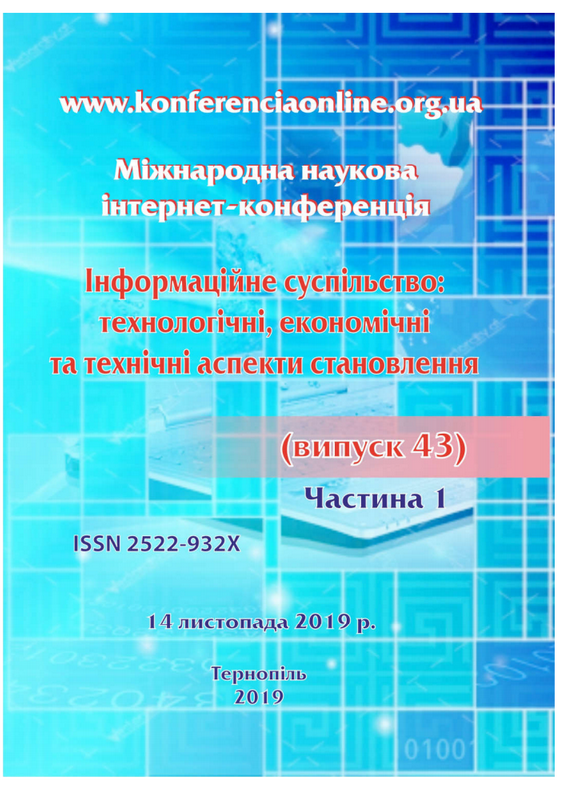
\includegraphics[width=1\textwidth, height=1.3\textwidth]{article-1}
\newpage

\includegraphics[width=1\textwidth, height=1.3\textwidth]{article-2}
\newpage
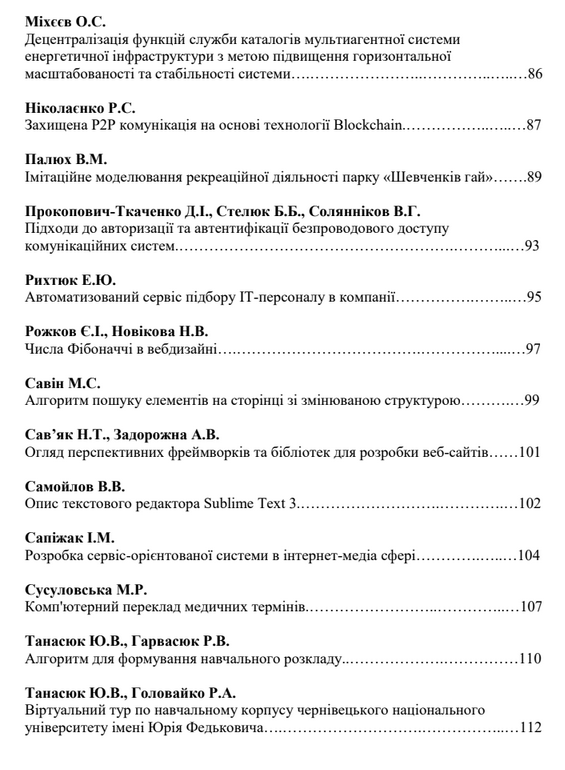
\includegraphics[width=1\textwidth, height=1.3\textwidth]{article-3}
\newpage

\includegraphics[width=1\textwidth, height=1.3\textwidth]{article-4}
\newpage
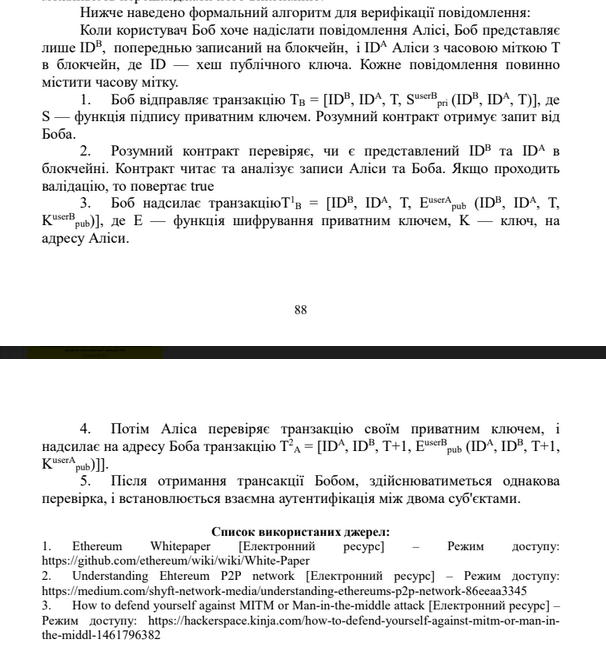
\includegraphics[width=1\textwidth, height=1.3\textwidth]{article-5}
\end{document}